% Author: Alfredo Sánchez Alberca (asalber@ceu.es)
%----------------------------------------------------------------------------------------
%    DOCUMENT CLASS
%----------------------------------------------------------------------------------------

\documentclass[11pt,a4paper,openright]{book}
%----------------------------------------------------------------------------------------
%	PACKAGES AND OTHER DOCUMENT CONFIGURATIONS
%----------------------------------------------------------------------------------------

% Language settings
\usepackage{polyglossia}
\setdefaultlanguage{english}

% Margins and layout
\usepackage[top=3cm, bottom=3cm, left=2.54cm, right=2.54cm]{geometry}

% Font settings
\usepackage{mathpazo} 
\usepackage{fontspec}
\setmainfont[Ligatures=TeX]{TeX Gyre Pagella}
%\usepackage{unicode-math}
%\setmathfont[math-style=ISO, bold-style=ISO, vargreek-shape=TeX]{TeX Gyre Pagella Math}

% Color
\usepackage{xcolor} % Required for specifying colors by name
\definecolor{color1}{RGB}{5,161,230}
\definecolor{color2}{RGB}{238,50,36}
\definecolor{ocre}{RGB}{243,102,25} % Define the orange color used for highlighting throughout the book
\definecolor{blueceu}{RGB}{5,161,230} % Blue color of CEU logo
\definecolor{greenceu}{RGB}{185,209,16} % Green color of CEU logo
\definecolor{redceu}{RGB}{238,50,36} % Red color of CEU logo
\definecolor{grayceu}{RGB}{111,107,83} % Gray color of CEU logo
\definecolor{coral}{rgb}{1,0.5,0.31} % Orange color for graphics
\definecolor{royalblue1}{rgb}{0.28,0.46,1} % Blue color for graphics
\definecolor{mygreen}{rgb}{0,0.8,0} % Green color for graphics
\definecolor{chaptergrey}{RGB}{5,161,230} % Blue color of CEU logo

% Math support
\usepackage{amsmath} 

% Line breaking
\usepackage{microtype} 
\setlength{\emergencystretch}{2em}

% Graphics
\usepackage{graphicx}
\usepackage{tikz} 
\usepackage{eso-pic} % Required for specifying an image background in the title page

% Arrays and tables
\usepackage{array}
\usepackage{multirow}
\usepackage{multicol}
\usepackage{colortbl}
\usepackage{booktabs}
\newcommand{\tcrule}{\arrayrulecolor{color1!50!white}\toprule}
\newcommand{\mcrule}{\arrayrulecolor{color1!50!white}\midrule}
\newcommand{\bcrule}{\arrayrulecolor{color1!50!white}\bottomrule}

% Captions
\usepackage[margin=20pt, font=small, labelfont=bf, labelsep=endash]{caption}

% Floating figures
\usepackage{subfigure}

% Lists
\usepackage[shortlabels]{enumitem} % Customize lists
%\setlist{nolistsep} % Reduce spacing between bullet points and numbered lists
\setlist[description]{style=sameline,leftmargin=0cm}

\makeatletter
\let\savees@listquot\es@listquot
\def\es@listquot{\protect\savees@listquot}
\makeatletter

\renewcommand{\theenumiii}{\arabic{enumiii}}

% Flush floating 
\usepackage{afterpage}

% Creative common icons
\usepackage[scale=2]{ccicons}

% hyperlinks
\usepackage{hyperref}
\hypersetup{
pdfauthor = {Alfredo S\'anchez Alberca},
pdftitle = {Calculus with Derive},
pdfsubject = {Calculus},
pdfkeywords = {Maths, Calculus, Derive},
pdfcreator = {XeLaTeX with hyperref package},
pdfproducer = {pdfLaTeX},
colorlinks = true,
linkcolor = red,          % color of internal links
citecolor = green,        % color of links to bibliography
filecolor = magenta,      % color of file links
urlcolor = magenta,          % color of external links
}
%\usepackage{breakurl}

% Indentation
%\setlength\parindent{0pt}

% Control of widow orphan lines
\clubpenalty=10000
\widowpenalty=10000 

%Code listing formatting
\usepackage{listings}
\lstdefinelanguage{morejava}{morekeywords={String}}
\definecolor{vollgrau}{rgb}{0.9,0.9,0.9}
\definecolor{colKeys}{rgb}{0,0,1}
\definecolor{colIdentifier}{rgb}{0,0,0}
\definecolor{colComments}{rgb}{1,0.5,0}
\definecolor{colString}{rgb}{0,0.5,0}
\definecolor{colbackground}{rgb}{0.9,0.9,1}


% Set short or long depending on the version desired
% \usepackage[corto]{optional}

%----------------------------------------------------------------------------------------
%	SECTIONS AND SUBSECTIONS
%----------------------------------------------------------------------------------------
%\titleformat*{\section}{\Huge}
%\titleformat*{\subsection}{\Large}


% Chapter and section formatting 
\usepackage[rigidchapters,explicit]{titlesec}
\setlength{\fboxsep}{5pt}
\newlength{\titulolength}
\setlength{\titulolength}{\textwidth} 
\addtolength{\titulolength}{-2\fboxsep}
\addtolength{\titulolength}{-2\fboxrule}
\titleformat{\chapter}[display]
{\bfseries\sffamily}
{\filleft \mdseries \LARGE \color{blueceu} Practice \Huge\thechapter}
{0.5ex}
{\colorbox{blueceu}{\parbox[t]{\titulolength}{\rule{0mm}{10mm}\Huge\sffamily\filleft\textcolor{white}{#1}}}}
\titleformat{\section}{\normalfont\Large\bfseries\color{blueceu}}{\arabic{section}}{1em}{#1}
\titleformat{\subsection}{\normalfont\large\bfseries\color{blueceu}}{\arabic{section}.\arabic{subsection}}{1em}{#1}
\titleformat{\subsubsection}{\normalfont\normalsize\bfseries\color{blueceu}}{\arabic{section}.\arabic{subsection}.\arabic{subsubsection}}{0.5em}{#1}
\titlespacing{\chapter}{0pt}{0pt}{30ex}
\titlespacing{\section}{0pt}{8ex}{4ex}

%----------------------------------------------------------------------------------------
%	MAIN TABLE OF CONTENTS
%----------------------------------------------------------------------------------------

% \usepackage{titletoc} % Required for manipulating the table of contents
% 
% \contentsmargin{0cm} % Removes the default margin
% % Chapter text styling
% \titlecontents{chapter}[1.25cm] % Indentation
% {\addvspace{15pt}\large\bfseries} % Spacing and font options for chapters
% {\color{gray}\contentslabel[\Large\thecontentslabel.]{1.25cm}} % Chapter number
% {}  
% {\color{gray}\bfseries\hfill\thecontentspage} % Page number
% % Section text styling
% \titlecontents{section}[1.25cm] % Indentation
% {\addvspace{5pt}\bfseries} % Spacing and font options for sections
% {\contentslabel[\thecontentslabel]{1.25cm}} % Section number
% {}
% {\hfill\color{black}\thecontentspage} % Page number
% []
% % Subsection text styling
% \titlecontents{subsection}[1.25cm] % Indentation
% {\addvspace{1pt}\small} % Spacing and font options for subsections
% {\contentslabel[\thecontentslabel]{1.25cm}} % Subsection number
% {}
% {\;\titlerule*[.5pc]{.}\;\thecontentspage} % Page number
% [] 

%----------------------------------------------------------------------------------------
%	MINI TABLE OF CONTENTS IN CHAPTER HEADS
%----------------------------------------------------------------------------------------

% % Section text styling
% \titlecontents{lsection}[0em] % Indendating
% {\footnotesize\sffamily} % Font settings
% {}
% {}
% {}
% 
% % Subsection text styling
% \titlecontents{lsubsection}[.5em] % Indentation
% {\normalfont\footnotesize\sffamily} % Font settings
% {}
% {}
% {}
 
%----------------------------------------------------------------------------------------
%	PAGE HEADERS
%----------------------------------------------------------------------------------------

% Headings and footers
\usepackage{fancyhdr}
\pagestyle{fancy}
\fancyhead{}
\renewcommand{\chaptermark}[1]{\markboth{\thechapter.\ #1}{}}
\fancyhead[LE]{\scshape Calculus with Derive}
\fancyhead[RO]{\sffamily\slshape \leftmark}
\renewcommand{\headrulewidth}{0pt}
\renewcommand{\floatpagefraction}{.8}
\renewcommand{\textfraction}{.1}


% \usepackage{fancyhdr} % Required for header and footer configuration
% 
% \pagestyle{fancy}
% \renewcommand{\chaptermark}[1]{\markboth{\color{grayceu}\sffamily\normalsize\textit{#1}}{}} % Chapter text font
% % settings
% %\renewcommand{\sectionmark}[1]{\markright{\color{grayceu}\sffamily\normalsize\textit{\thesection\hspace{5pt}#1}}{}} %
% % Section text font settings
% \fancyhf{} \fancyfoot[LE,RO]{\normalsize\thepage} % Font setting for the page number in the footer
% \fancyhead[RE]{{\color{grayceu}\sffamily\normalsize\textit{Pr�cticas de Bioestad�stica con R and RKTeaching}}} % Print the nearest
% % section name on the left side of odd pages
% \fancyhead[LO]{\leftmark} % Print the current chapter name on the right side of even pages
% \renewcommand{\headrulewidth}{0pt} % Removes the rule in the header
% \addtolength{\headheight}{2.5pt} % Increase the spacing around the header slightly
% \renewcommand{\footrulewidth}{0pt} % Removes the rule in the footer
% \fancypagestyle{plain}{\fancyhead{}\renewcommand{\headrulewidth}{0pt}} % Style for when a plain pagestyle is specified
% 
% % Removes the header from odd empty pages at the end of chapters
% \makeatletter
% \renewcommand{\cleardoublepage}{
% \clearpage\ifodd\c@page\else
% \hbox{}
% \vspace*{\fill}
% \thispagestyle{empty}
% \newpage
% \fi}


%----------------------------------------------------------------------------------------
%	THEOREM STYLES
%----------------------------------------------------------------------------------------

\usepackage{amsthm} % For including math equations, theorems, symbols, etc

\newcommand{\intoo}[2]{\mathopen{]}#1\,;#2\mathclose{[}}
\newcommand{\ud}{\mathop{\mathrm{{}d}}\mathopen{}}
\newcommand{\intff}[2]{\mathopen{[}#1\,;#2\mathclose{]}}
\newtheorem{notation}{Notation}[chapter]

\newtheoremstyle{blueceu} % Theorem style name
{7pt} % Space above
{7pt} % Space below
{\normalfont} % Body font
{} % Indent amount
{\small\bf\sffamily\color{blueceu}} % Theorem head font
{\;\;} % Punctuation after theorem head
{0.25em} % Space after theorem head
{\small\sffamily\color{blueceu}\thmname{#1}\thmnumber{\@ifnotempty{#1}{ }\@upn{#2}} % Theorem text (e.g. Theorem 2.1)
\thmnote{\ {\the\thm@notefont\sffamily\bfseries\color{blueceu}--- #3.}}} % Optional theorem note
\renewcommand{\qedsymbol}{$\blacksquare$} % Optional qed square

\newtheoremstyle{blacknumex} % Theorem style name
{7pt} % Space above
{7pt} % Space below
{\normalfont} % Body font
{} % Indent amount
{\small\bf\sffamily} % Theorem head font
{\;\;} % Punctuation after theorem head
{0.25em} % Space after theorem head
{\small\sffamily{\tiny\ensuremath{\blacksquare}}\ \thmname{#1}\thmnumber{\@ifnotempty{#1}{ }\@upn{#2}} % Theorem text (e.g. Theorem 2.1)
\thmnote{\ {\the\thm@notefont\sffamily\bfseries--- #3.}}} % Optional theorem note

\newtheoremstyle{blacknum} % Theorem style name
{7pt} % Space above
{7pt} % Space below
{\normalfont} % Body font
{} % Indent amount
{\small\bf\sffamily} % Theorem head font
{\;\;} % Punctuation after theorem head
{0.25em} % Space after theorem head
{\small\sffamily\thmname{#1}\thmnumber{\@ifnotempty{#1}{ }\@upn{#2}} % Theorem text (e.g. Theorem 2.1)
\thmnote{\ {\the\thm@notefont\sffamily\bfseries--- #3.}}} % Optional theorem note

\newtheoremstyle{example} % Theorem style name
{7pt} % Space above
{7pt} % Space below
{\normalfont} % Body font
{} % Indent amount
{\small\bf\sffamily} % Theorem head font
{\;\;} % Punctuation after theorem head
{0.25em} % Space after theorem head
{\small\sffamily\thmname{#1} % Theorem text (e.g. Theorem 2.1)
\thmnote{\ {\the\thm@notefont\sffamily\bfseries--- #3.}}} % Optional theorem note

\newtheoremstyle{indication} % Theorem style name
{-5pt} % Space above
{7pt} % Space below
{\normalfont} % Body font
{-28pt} % Indent amount
{\bf} % Theorem head font
{\kern-11.5pt} % Punctuation after theorem head
{20pt} % Space after theorem head
{\begin{tikzpicture}
\draw node [fill=blueceu,opacity=1,inner sep=1pt] {\makebox[17pt][c]{
\includegraphics[scale=0.3]{img/bulb}}}; \end{tikzpicture}} % Theorem text (e.g. Theorem 2.1)

\makeatother

% Defines the theorem text style for each type of theorem to one of the three styles above
\theoremstyle{ocrenum}
\newtheorem{exerciseT}{Exercise}[chapter]
\theoremstyle{blacknumex}
\newtheorem{exampleT}{Example}[chapter]
%\theoremstyle{blacknum}
\theoremstyle{blueceu}
\newtheorem{vocabulary}{Vocabulary}[chapter]
\newtheorem{definitionT}{Definition}[chapter]
\newtheorem{theoremT}{Theorem}[chapter]
\newtheorem{corolary}{Corolary}[chapter]
\theoremstyle{indication}
\newtheorem{indicationT}{Indication}
%\theoremstyle{example}
%\newtheorem{ejemplo}{Ejemplo}

%----------------------------------------------------------------------------------------
%	DEFINITION OF COLORED BOXES
%----------------------------------------------------------------------------------------

\RequirePackage[framemethod=default]{mdframed} % Required for creating the theorem, definition, exercise and corollary boxes

% Theorem box
\newmdenv[skipabove=7pt,
skipbelow=7pt,
backgroundcolor=black!5,
linecolor=ocre,
innerleftmargin=5pt,
innerrightmargin=5pt,
innertopmargin=5pt,
leftmargin=0cm,
rightmargin=0cm,
innerbottommargin=5pt]{tBox}

% Exercise box	  
\newmdenv[skipabove=7pt,
skipbelow=7pt,
rightline=false,
leftline=true,
topline=false,
bottomline=false,
backgroundcolor=ocre!10,
linecolor=ocre,
innerleftmargin=5pt,
innerrightmargin=5pt,
innertopmargin=5pt,
innerbottommargin=5pt,
leftmargin=0cm,
rightmargin=0cm,
linewidth=4pt]{eBox}	

% Definition box
\newmdenv[skipabove=10pt,
skipbelow=10pt,
rightline=false,
leftline=true,
topline=false,
bottomline=false,
linecolor=ocre,
innerleftmargin=5pt,
innerrightmargin=5pt,
innertopmargin=0pt,
leftmargin=0cm,
rightmargin=0cm,
linewidth=4pt,
innerbottommargin=0pt]{dBox}	

% Corollary box
\newmdenv[skipabove=7pt,
skipbelow=7pt,
rightline=false,
leftline=true,
topline=false,
bottomline=false,
linecolor=gray,
backgroundcolor=black!5,
innerleftmargin=5pt,
innerrightmargin=5pt,
innertopmargin=5pt,
leftmargin=0cm,
rightmargin=0cm,
linewidth=4pt,
innerbottommargin=5pt]{cBox}	

% Indication box
\newmdenv[skipabove=7pt,
skipbelow=7pt,
rightline=false,
leftline=true,
topline=false,
bottomline=false,
linecolor=blueceu,
backgroundcolor=black!5,
innerleftmargin=5pt,
innerrightmargin=5pt,
innertopmargin=5pt,
leftmargin=0pt,
rightmargin=0pt,
linewidth=4pt,
innerbottommargin=5pt]{iBox}		  
		  			  


% Creates an environment for each type of theorem and assigns it a theorem text style from the "Theorem Styles" section above and a colored box from above
\newenvironment{theorem}{\begin{tBox}\begin{theoremT}}{\end{theoremT}\end{tBox}}
\newenvironment{exercise}{\begin{eBox}\begin{exerciseT}}{\hfill{\color{ocre}\tiny\ensuremath{\blacksquare}}\end{exerciseT}\end{eBox}}				  
\newenvironment{definition}{\begin{dBox}\begin{definitionT}}{\end{definitionT}\end{dBox}}	
\newenvironment{example}{\begin{exampleT}}{\hfill{\tiny\ensuremath{\blacksquare}}\end{exampleT}}		
\newenvironment{corollary}{\begin{cBox}\begin{corollaryT}}{\end{corollaryT}\end{cBox}}	
\newenvironment{indication}{\begin{iBox}\begin{indicationT}}{\end{indicationT}\end{iBox}}	

%----------------------------------------------------------------------------------------
%	REMARK ENVIRONMENT
%----------------------------------------------------------------------------------------

%\newenvironment{remark}{\par\vskip10pt\small % Vertical white space above the remark and smaller font size
%\begin{list}{}{
%\leftmargin=35pt % Indentation on the left
%\rightmargin=25pt}\item\ignorespaces % Indentation on the right
%\makebox[-2.5pt]{\begin{tikzpicture}[overlay]
%\node[draw=ocre!60,line width=1pt,circle,fill=ocre!25,font=\sffamily\bfseries,inner sep=2pt,outer sep=0pt] at (-15pt,0pt){\textcolor{ocre}{R}};\end{tikzpicture}} % Orange R in a circle
%\advance\baselineskip -1pt}{\end{list}\vskip5pt} % Tighter line spacing and white space after remark

% %----------------------------------------------------------------------------------------
% %	SECTION NUMBERING IN THE MARGIN
% %----------------------------------------------------------------------------------------
% 
% \makeatletter
% %\renewcommand{\@seccntformat}[1]{\llap{\textcolor{grayceu}{\csname the#1\endcsname.}\hspace{1em}}}                    
% \renewcommand{\section}{
% 	\@startsection{section}{1}{\z@}
% 	{-4ex \@plus -1ex \@minus -.4ex}{1ex \@plus.2ex }
% 	{\normalfont\LARGE}
% }
% \renewcommand{\subsection}{
% 	\@startsection{subsection}{2}{\z@}
% 	{-3ex \@plus -0.1ex \@minus -.4ex}{0.5ex \@plus.2ex }
% 	{\normalfont\Large}
% }
% \renewcommand{\subsubsection}{
% 	\@startsection{subsubsection}{3}{\z@}
% 	{-2ex \@plus -0.1ex \@minus -.2ex}{0.2ex \@plus.2ex }
% 	{\normalfont\large}
% }                        
% \renewcommand{\paragraph}{
% 	\@startsection{paragraph}{4}{\z@}
% 	{-2ex \@plus-.2ex \@minus .2ex}{0.1ex}
% 	{\normalfont\bfseries}
% }
% 
% \def\thechapter{\arabic{chapter}}
% \def\thesection{\thechapter.\arabic{section}.}
% \def\thesubsection{\thesection\arabic{subsection}.}
% \def\thesubsubsection{\thesubsection\arabic{section}.}
% 
% %----------------------------------------------------------------------------------------
% %	CHAPTER HEADINGS
% %----------------------------------------------------------------------------------------
% %\newcommand{\thechapterimage}{}
% %\newcommand{\chapterimage}[1]{\renewcommand{\thechapterimage}{#1}}
% \def\@makechapterhead#1{
% \thispagestyle{empty}
% {
% \ifnum \c@secnumdepth >\m@ne
% \if@mainmatter
% \startcontents
% \begin{tikzpicture}[remember picture,overlay]
% % \node at (current page.north west)
% % {\begin{tikzpicture}[remember picture,overlay]
% % 
% % %\node[anchor=north west] at (-4pt,-27.5mm) {\includegraphics[width=\paperwidth]{\thechapterimage}};
% % %Commenting the 3 lines below removes the small contents box in the chapter heading
% % % \draw[fill=white,opacity=.6] (30mm,-30mm) rectangle (9cm,-9cm);
% % % \node[anchor=north west] at (30mm,-30mm) {\parbox[t][9cm][t]{5.5cm}{\huge\bfseries\flushleft \printcontents{l}{1}{\setcounter{tocdepth}{2}}}};
% % % \draw[anchor=west] (5cm,-11cm) node [rounded corners=25pt,fill=white,opacity=.7,inner sep=15.5pt]{\huge\sffamily\bfseries\textcolor{black}{\vphantom{plPQq}\makebox[20cm]{}}};
% \draw[anchor=north west, fill=black] (0mm,50mm) rectangle (1pt,10mm);
% \draw[anchor=north west] (0cm,20mm) node {\scalebox{1.5}{\Huge{\textcolor{grayceu}\thechapter}}}; 
% %\draw[anchor=west] (0cm,0cm) node {\Huge{#1}}; 
% \end{tikzpicture}
% \par\vspace*{2cm}
% {\Huge #1}
% \par\vspace*{1cm}
% % \end{tikzpicture}}\par\vspace*{230\p@}
% }}
% \def\@makeschapterhead#1{
% \thispagestyle{empty}
% {
% \ifnum \c@secnumdepth >\m@ne
% \if@mainmatter
% \startcontents
% \begin{tikzpicture}[remember picture,overlay]
% % \node at (current page.north west)
% % {\begin{tikzpicture}[remember picture,overlay]
% % \node[anchor=north west] at (-4pt,-27.5mm) {\includegraphics[width=\paperwidth]{\thechapterimage}};
% % \draw[anchor=west] (5cm,-11cm) node [rounded corners=25pt,fill=white,opacity=.7,inner sep=15.5pt]{\huge\sffamily\bfseries\textcolor{black}{\vphantom{plPQq}\makebox[20cm]{}}};
% % \draw[anchor=west] (5cm,-11cm) node [rounded corners=25pt,inner sep=15.5pt]{\huge\sffamily\bfseries\textcolor{black}{#1\vphantom{plPQq}\makebox[20cm]{}}};
% % \end{tikzpicture}};
% % \end{tikzpicture}}\par\vspace*{230\p@}
% %\draw[anchor=west] (0cm,0cm) node {\Huge{#1}}; 
% \end{tikzpicture}
% {\Huge #1}
% \par\vspace*{1cm}
% }}
% \makeatother

 % Insert the commands_book.tex file which contains the majority of the structure behind
% the template

%----------------------------------------------------------------------------------------
%	COMMANDS FOR INDICATIONS
%----------------------------------------------------------------------------------------
\usepackage{menukeys}
\newmenucolortheme{mycolors}{named}{white}{color1}{black}
\changemenucolortheme{menus}{mycolors}
\renewmenumacro{\menu}[>]{menus}
%\newmenustylesimple*{botonstyle}{\textbf{\CurrentMenuElement}}
%\renewmenumacro{\keys}{botonstyle}
\newcommand{\button}[1]{\textsf{\small #1}}
\newcommand{\option}[1]{\textsf{\small #1}}
\newcommand{\mtab}[1]{\textsf{\small #1}}
\newcommand{\field}[1]{\textsf{\small #1}}
\newcommand{\command}[1]{\texttt{#1}}
\newcommand{\variable}[1]{\textsf{\small #1}}
\newcommand{\result}[1]{\texttt{#1}}

% OTHERS
\newcommand{\resetcounters}{\setcounter{page}{1} \setcounter{section}{0} \setcounter{footnote}{0} \setcounter{figure}{0} \setcounter{table}{0}}


%========================================================================================
%   DOCUMENT BODY
%========================================================================================
\begin{document}
\frontmatter 
% Add two blank pages at the begining
%\null\thispagestyle{empty}\newpage
%\null\thispagestyle{empty}\newpage
%----------------------------------------------------------------------------------------
%	TITLE PAGE
%----------------------------------------------------------------------------------------
\begin{titlepage}
\thispagestyle{empty}
\vspace*{7cm}
\par

% Book title
\begin{center}
\normalfont\fontsize{30}{30}\selectfont
{\bfseries \color{blueceu}Calculus with Derive}
\end{center}
\vspace{1cm}

% Authors names
\begin{center}
\Large
\begin{tabular}{c}
%Pablo Ares Gastesi (\url{pablo.aresgastesi@ceu.es})\\
Juan Carlos Garro Garro (\url{garro.eps@ceu.es})\\
Euardo López Ramírez (\url{elopez@ceu.es})\\
José Rojo Montijano (\url{jrojo.eps@ceu.es})\\
Anselmo Romero Limón (\url{arlimon@ceu.es})\\
Alfredo Sánchez Alberca (\href{mailto:asalber@ceu.es}{asalber@ceu.es})\\
Susana Victoria Rodríguez (\url{victoria.eps@ceu.es})
\end{tabular}

\medskip 
Department of Applied Math and Statistics\\ CEU San Pablo\\[1cm]
\medskip 
September 2016

\vspace{1cm}

\includegraphics[height=3cm]{img/logo_uspceu}
\end{center}
\vfill
\end{titlepage} 
%\begin{titlepage}
\AddToShipoutPictureBG*{\includegraphics[width=\paperwidth,height=\paperheight]{img/portada}}
\clearpage
\thispagestyle{empty}
\end{titlepage}

\null\newpage
\thispagestyle{empty}

\null\newpage
\thispagestyle{empty}
%\thispagestyle{empty}
\vspace*{7cm}
\par

% Book title
\begin{center}
\normalfont\fontsize{30}{30}\selectfont
\textsc{\color{blueceu}Bioestadística Aplicada\\ con R and RKTeaching}
\end{center}
\par  
%\vspace*{5mm}
%\hrule
\vspace*{3cm}
% Authors names
\begin{center}
\Large
\begin{tabular}{c}
%Santiago Angulo Díaz-Parreño (\url{sangulo@ceu.es})\\
%Euardo López Ramírez (\url{elopez@ceu.es})\\
%José Rojo Montijano (\url{jrojo.eps@ceu.es})\\
%Anselmo Romero Limón (\url{arlimon@ceu.es})\\
Alfredo Sánchez Alberca\\
\url{asalber@ceu.es}\\
\url{http://aprendeconalf.es}
\end{tabular}
\end{center}

\vspace*{1cm}
\begin{center}
Septiembre de 2014
\end{center}
\par
\vfill
%\includegraphics[scale=0.3]{img/logo_uspceu_01}

\newpage 
 
%----------------------------------------------------------------------------------------
%	COPYRIGHT PAGE
%----------------------------------------------------------------------------------------
\thispagestyle{empty}
\null
\vfill
\hrule depth 3pt
\smallskip
\sffamily

\noindent \textbf{Calculus with Derive}\\
Alfredo Sánchez Alberca (asalber@ceu.es) 

\bigskip
% Creative Commons license terms
{\Large \textbf{License terms \normalsize \ccLogo}}
\medskip

\small
This work is licensed under an Attribution-NonCommercial-ShareAlike 4.0 International Creative Commons License. 
\url{http://creativecommons.org/licenses/by-nc-sa/4.0/}

You are free to: 

\begin{itemize}
\item Share -- copy and redistribute the material in any medium or format
\item Adapt -- remix, transform, and build upon the material
\end{itemize}

Under the following terms:
\begin{center}
\begin{tabular}{cp{0.8\textwidth}}
\ccAttribution &  \textbf{Attribution}. You must give appropriate credit, provide a link
to the license, and indicate if changes were made. You may do so in any reasonable manner, but not in any way that
suggests the licensor endorses you or your use.\\ 
\ccNonCommercialEU & \textbf{NonComercial}. You may not use the material for commercial purposes.\\ 
\ccShareAlike & \textbf{ShareAlike}. If you remix, transform, or build upon the material, you must distribute
your contributions under the same license as the original.
\end{tabular}
\end{center}

No additional restrictions — You may not apply legal terms or technological measures that legally restrict others from
doing anything the license permits.


\normalfont
\newpage

%----------------------------------------------------------------------------------------
%	TABLE OF CONTENTS
%----------------------------------------------------------------------------------------
%\chapterimage{img/chapter_head.png} % Table of contents heading image
{\pagestyle{plain} % No headers
%\input{registro}
\tableofcontents\thispagestyle{empty}
  % Print the table of contents itself
\cleardoublepage % Forces the first chapter to start on an odd page so it's on the right
}

\mainmatter 
%----------------------------------------------------------------------------------------
%	CHAPTERS 
%----------------------------------------------------------------------------------------
% % Author: Alfredo Sánchez Alberca (asalber@ceu.es)
\chapter{Introducction to Derive}

\section{Introduction}
In the last decades, the computational power of computers have converted them in powerful tools for disciplines that, as Mathematics, require a large amount of complex computations.

Derive$^{\textsf{\textregistered}}$
\renewcommand{\thefootnote}{\fnsymbol{footnote}}\footnote{These practices are based on version 6.1 of Derive$^{\textregistered}$ for Windows.} is one of the most used programs for doing numerical and symbolic computations.  

Beyond their capabilities for the numerical, vectorial and matrix calculus, it also makes graphical representations. 
This allows to solve a lot of problems of Algebra, Analysis, Calculus, Geometry and even Statistics. 
The advantage of Derive versus other software as Mathematica, Mapple or MATLAB, is its simplicity, what makes it suitable for teaching Maths. 

\begin{center}
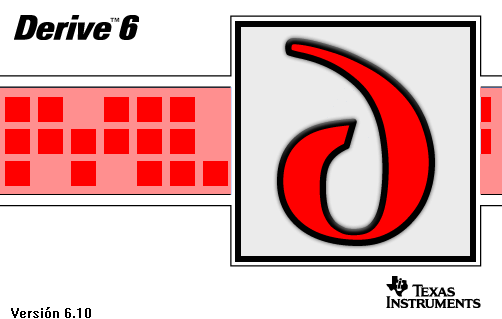
\includegraphics[scale=0.6]{img/introduction/introduction}
\end{center}


The goal of this practice is to introduce the basic usage of this program to the student. 


\section{Basic functionalities}
\subsection*{Starting the program}
As any other Windows applications, to start the program you have to click the \menu{Windows start} button and then select \menu{All the programs > Derive 6} or simply double click the desktop shortcut if there is one. 


\begin{center}
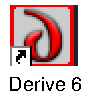
\includegraphics[scale=0.4]{img/introduction/derive_icon}
\end{center}

When the program starts, the main window, that is known as \emph{Algebra window} is shown (figure \ref{g:main}).

\begin{figure}[h!]
\begin{center}
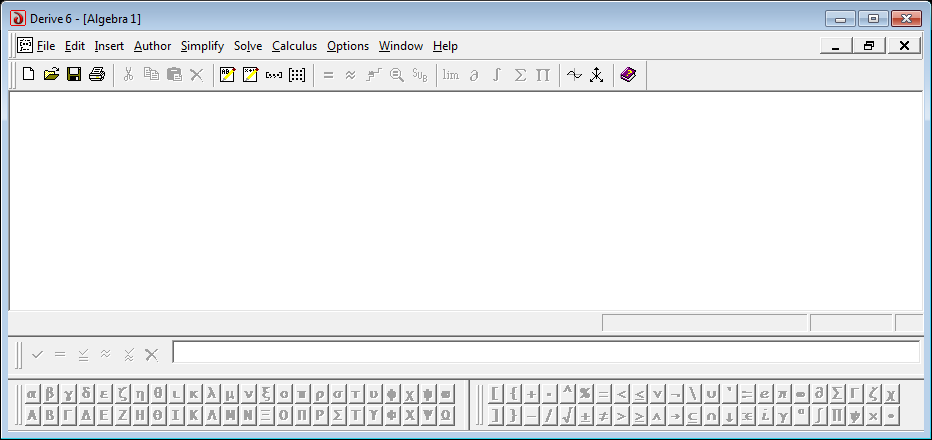
\includegraphics[width=\textwidth]{img/introduction/algebra_window}
\caption{Algebra window of Derive} \label{g:main} 
\end{center}
\end{figure}


The Algebra window has a title bar, a menu bar with menus for all the computations that Derive can performs (limits, derivatives, integrals, graphical representations, etc.), a tool bar with buttons for the main computations, the working area that contains the mathematical expressions that we are working with, the expression editor bar to enter mathematical expressions, the Greek letters and symbols button bar with Greek letters and symbols to enter in expressions and the status bar that shows what is the program doing at any moment. 

\subsection*{Expression edition}
Before doing any computation with a mathematical expression we have to enter it. 

\subsection*{Entering a mathematical expression}
To enter a mathematical expression we use the expression editor bar (figure~\ref{g:expression-editor}), that usually appears at the bottom of the Algebra widows, over the Greeks letters and symbols bar.

\begin{figure}[h!]
\begin{center}

\includegraphics[scale=0.6]{img/introduction/expression_editor}
\caption{Expression editor bar.} \label{g:expression-editor} 
\end{center} 
\end{figure}


In the expression editor bar we can write numbers, letters (that are variables) and symbols and arithmetic and logic operators. 
The most common operators are shown in the table below. 
You can also enter any Greek letter or symbol of the Greek letters and symbols button bar, just clicking on it.


\begin{center}
\begin{tabular}{cc}
\tcrule
\textbf{Symbol} & \textbf{Operator} \\
\texttt{+} & addition \\
\texttt{-} & subtraction \\
\texttt{*} & product \\
\texttt{/} & division \\
\texttt{\^{}} & power \\
\bcrule
\end{tabular}
\end{center}


Operators have different priorities when Derive evaluates a expression. 
First it evaluates functions and constants, second powers, third products and quotients (from left to right) and finally sums and subtractions (from left to right). 
You have to take into account this priority or use parenthesis to force a subexpression to be evaluated before the rest. 
In the following example you have different expressions and what Derive interprets for each of them

\begin{center}\renewcommand{\arraystretch}{2}
\begin{tabular}{cc}
\tcrule
\textbf{Entered expression} & \textbf{Evaluated expression} \\
\texttt{4x-1/x-5} & $4x-\dfrac{1}{x}-5$ \\
\texttt{(4x-1)/x-5} & $\dfrac{4x-1}{x}-5$ \\
\texttt{4x-1/(x-5)} & $4x-\dfrac{1}{x-5}$ \\
\texttt{(4x-1)/(x-5)} & $\dfrac{4x-1}{x-5}$ \\
\bcrule
\end{tabular}
\end{center}

After entering a expression and pressing \button{Enter}, the expression is shown in the working area of the Algebra window, labelled with a tag \verb"#" and a number, such as is shown in the figure~\ref{g:expressions}. 
After that we can reference that expression using its label instead of typing again the expression. 

We can select any expression of the Algebra window click on it. 
If you click several times on the same expression you can select different subexpressions. 
It is also possible to select several consecutive expressions in a block clicking on the first expression and dragging the cursor to the last. 

A useful key is \texttt{F3} that allow entering the selected expression or subexpression in the expression editor bar.

\subsubsection*{Modifying a expression}
Once a expression has been entered, we can modify it clicking on the expression and selecting the menu \menu{Edit > Expression}. 
The expression will be entered in the expression editor bar where you can change whatever you want. 
After making the changes, don't forget to press \button{Enter}. 

\subsubsection*{Removing expressions}
To remove a expression form the working area of the Algebra window, it is enough to select the expression and then press the \button{Supr} key or select the menu \menu{Edit > Delete}.
After removing a expression the labels of the other expressions are renumbered automatically. 
It is also possible to remove blocks of consecutive expressions. 

\textbf{Important!}: If we remove a expression by mistake, it is possible to recover it with the menu \menu{Edit > Undelete}.

\subsubsection*{Rearranging expressions}
It is possible to change the position of any expression in the working area of the Algebra window just clicking on it and, when the expression or block is selected, clicking again on it an dragging it to the new position.  
After arranging a expression the labels of the other expressions are renumbered automatically. 

\subsubsection*{Entering Comments}
The are two ways of entering comments in the working area of the Algebra window. 
The first one is in the expression editor bar, entering the text of the comment in double quotes.
If we proceed this way, the comment will be shown in the working area as any other expression, with its label. 
The second one is with the menu \menu{Insert > Text object}.
If we proceed this other way, the comment will be shown in the working area as an object without label. 

\subsubsection*{Naming variables}
By default Derive uses a single letter to represent variables. 
Thus, the expression \texttt{xy}, is not interpreted as a variable but as the product of variables $x$ and $y$.
Also by default, Derive does not distinguish between lowercase and uppercase letters.
For instance, Derive will interpret the same both if we write \command{cos(x)} or if we write \command{cos(X)}.
Nevertheless, it is possible to configure Derive to use more than one letter for variable names and to be case sensitive with the \menu{Options > Mode settings > Input}.

\subsubsection*{Defining constants and functions}
It is possible to define constants and functions with the operator \command{:=}.
To define a constant it is enough to type the name of the constant followed by \command{:=} and the value of the constant.
For example to define the gravitational constant we can write \command{g:=9.81}. 

To define a function, on the other hand, we have to type the name of the function followed by the list of variables separated by comma in brackets, then \command{:=} and the expression that defines the function. 
Thus, for instance, to define the function that measures the area of a triangle \command{a(b,h):=(b*h)/2} where \command{b} and \command{h} are the variables for the base and the height of the triangle respectively (see figure~\ref{g:expressions}).

With respect to the definition of constants and functions we must be aware of two important facts: 

\begin{itemize}
\item Any time we define a constant or function, the definition is active during all the working session, even if we remove the definition expression.
To remove a definition we have to redefine the constant or function but letting blank the expression after \command{:=}.
For example, to remove the definition of the gravitational constant we have to write \command{g:=}.

\item Derive is case sensitive to function names, so that \command{a(b,h)} and \command{A(b,h)} will be different functions.
\end{itemize}

\subsubsection*{Built-in constants and functions}
Derive has most of the constants and elementary functions used in Mathematics built-in. The syntax of some of them is shown in table ~\ref{t:elementary-functions}.

\begin{table}[h!]
\centering
\begin{tabular}{cl}
\tcrule
\textbf{Syntax} & \textbf{Constant or function} \\
\verb"#"\command{e} & Euler's number $e=2.71828\ldots$ \\
\command{pi} & The number $\pi=3.14159\ldots$ \\
\verb"#"\command{i} & The imaginary number $i=\sqrt{-1}$ \\
\command{inf} & Infinite $\infty$ \\
\command{exp(x)}  & Exponential function $e^x$ \\
\command{log(x,a)} & Logarithmic function with base $a$, $\log_a x$ \\
\command{ln(x)} & Natural logarithmic function $\ln x$ \\
\command{sqrt(x)} & Square root function $\sqrt{x}$ \\
\command{sin(x)} & Sine function $\sin x$ \\
\command{cos(x)} & Cosine function $\cos x$ \\
\command{tan(x)} & Tangent function $\tan x$ \\
\command{asin(x)} & Arcsine function $\arcsin x$ \\
\command{acos(x)} & Arccosine function $\arccos x$ \\
\command{atan(x)} & Arctangent function $\arctan x$ \\
\bcrule
\end{tabular}
\caption{Syntax of some predefined constants and functions.} \label{t:elementary-functions}
\end{table}

In some cases we can also use the symbols of the symbols button bar to refer to these constants.

To know all the built-in constants and functions of Derive we can use the menu \menu{Help > Online} and visit the section \textsf{Built-in Functions and Constants}.

\textbf{Important!}: In built-in functions Derive is not case sensitive.
For instance, the cosine function can be written \command{cos(x)}, \command{Cos(x)} or \command{COS(x)}.

\subsubsection*{Vectors and matrices}
Derive can also deal with vectors and matrices.
To enter a vector you can use the menu \menu{Author > Vector}.
Then enter the number of elements of the vector in the dialog shown and click the \button{OK} button. 
Finally enter the elements of the vector in the dialog shown and click again the \button{OK} button. 
Another way to enter vectors in the expression editor bar is to type their components separated by commas in square brackets. 
For instance, to enter the vector $(x,y,z)$ we write \command{[x,y,z]} (see the figure~\ref{g:expressions}).

To enter matrices we can use the menu \menu{Author > Matrix}.
Then enter the number of rows and columns of the matrix in the dialog shown and click the \button{OK} button. 
Finally enter the elements of the matrix in the dialog shown and click again the \button{OK} button. 

Another way to enter matrices in the expression editor bar is to type their row vectors separated by commas in square brackets. 
For instance, to enter the matrix
\[
\left(
\begin{array}{ccc}
 1 & 2 & 3 \\
 a & b & c \\
\end{array}
\right)
\]
we write \command{[[1,2,3],[a,b,c]]} (see the figure~\ref{g:expressions}).

\begin{figure}[h!]
\begin{center}
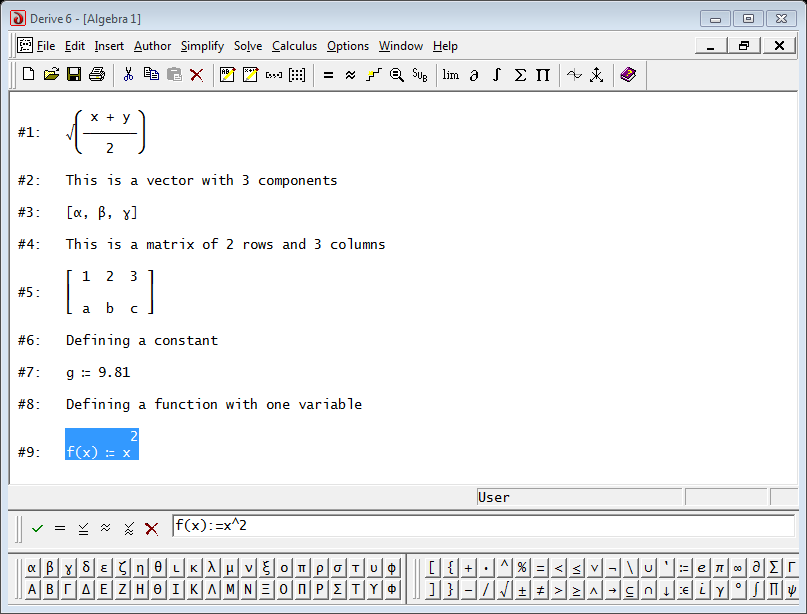
\includegraphics[width=0.8\textwidth]{img/introduction/expressions}
\caption{Different types of expressions in the Algebra window.}
\label{g:expressions}
\end{center}
\end{figure}


\subsection*{Simplifying expressions}
Derive has several ways to simplify expressions.
The simplest one is the basic simplification, that can be done with the menu \menu{Simplify > Basic}. 
This menu performs basic simplifications as, for instance, convert the expression $x+x$ in the expression $2x$. 
However, it doesn't allow to convert the binomial $(x+1)^2$ in $x^2+2x+1$, as it is not clear what of these expressions is simpler. 

To get the expansion of this binomial we can use the menu \menu{Simplify > Expand} that allow to expand a expression with respect to its variables.

On the contrary, if we want to get the binomial from the expanded form, we can use the menu \menu{Simplify > Factor} that allows to factor a expression with respect to its variables.

In any of these simplification types Derive woks in exact mode, what means that decimal numbers are expressed as fractions. 
To get the approximate value of an expression in a decimal form you can use the menu \menu{Simplify > Approximate}. 
This menu shows a dialog where we have to enter the number of decimal places that we want.

Finally, in any expression it is possible to substitute any variable by a value with the menu \menu{Simplify > Variable substitution}.
In the dialog shown you have to select the variable to substitute, enter the value for that variable in the field \field{New value} and click the button \button{OK}.


\subsection*{Graphical representations}
Derive can plot graphical representations in 2 and 3 dimensions.

\subsubsection*{2-dimensional graphical representations}
To represent a function or expression with one variable, we have to select the expression and then the menu \menu{Window > New 2D-plot window}.
This will open a new graphic window with two Cartesian axes ($x$ and $y$).
Finally, to show the graph of the expression in the Cartesian plane you have to select the menu \menu{Insert > Plot} or just click the corresponding button in the toolbar. 
Figure~\ref{g:2d-plot} shows an example of a 2-dimensional plot.

\begin{figure}[h!]
\begin{center}
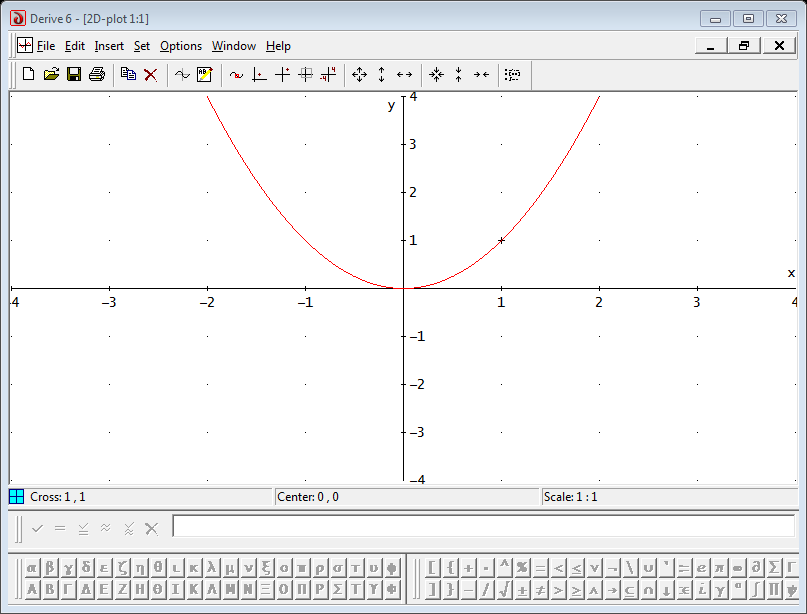
\includegraphics[width=0.8\textwidth]{img/introduction/2d-plot}
\caption{2-dimensional graphic window with the graph of a function.}
\label{g:2d-plot}
\end{center}
\end{figure}

If we want to show the plot in the Algebra window we can use the menu \menu{File > Embed}.

It is possible to represent more than one function in the same 2-dimensional graphic window. 

You can change from the Algebra window to the graphic window and vice versa selecting the corresponding window in the menu \menu{Window}.
However, when you are plotting several expressions is better to see the Algebra and graphic windows at the same time using the \menu{Window > Tile Vertically} (see figure~\ref{g:algebra-2d-plot}.

\begin{figure}[h!]
\begin{center}
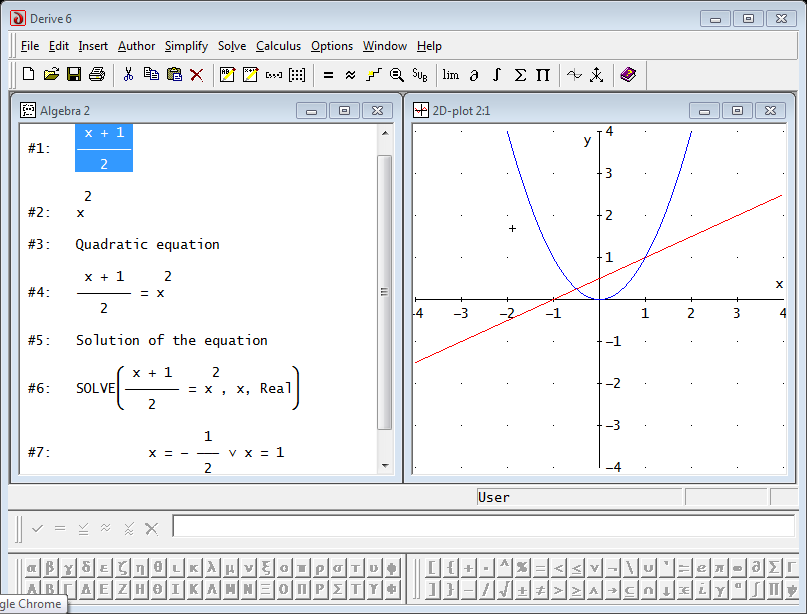
\includegraphics[width=0.8\textwidth]{img/introduction/algebra_2d-plot}
\caption{An Algebra and a 2-dimensional graphic window showed at the same time.} 
\label{g:algebra-2d-plot}
\end{center}
\end{figure}

\subsubsection*{Removing a plot}
To remove the last plot from a graphic window you can use the menu \menu{Edit > Delete plot > Last}. 
It is also possible to remove the first and all the plots but the last with the corresponding menus. 

\subsubsection*{Scaling a plot}
In the graphic window there are several menus and buttons to change the aspect of the plots. 

One of the most interesting actions is changing the scale of axes with the menu \menu{Set > Aspect Ratio}.
It is also possible to change the visible area of the plot with the menu \menu{Set > Plot Range > Minimum/Maximum}. 
In the dialog shown you have to enter the minimum and maximum values for every axis and click the button \button{OK}.


\subsubsection*{Tracing a plot}

In the 2-dimensional graphic windows there is a small cross that we change of position just clicking on a new position of the graphic window.
The coordinates of the cross are always shown in the bottom-left corner of the status bar.
If you press the \command{F3} key, the cross changes to a small square and passes to the \emph{trace mode}.
In this mode the square follows the trajectory of a graph using the arrow keys of the keyboard.
Use the left/right arrows to move the square to the left/right respectively and the up/down arrow to change the graph to follow when there are more than one plot. 
This can be helpful to see the value that takes a function in the graphic window or the points where two graphs intersect (see figure~\ref{g:trace-mode}.

\begin{figure}[h!]
\begin{center}
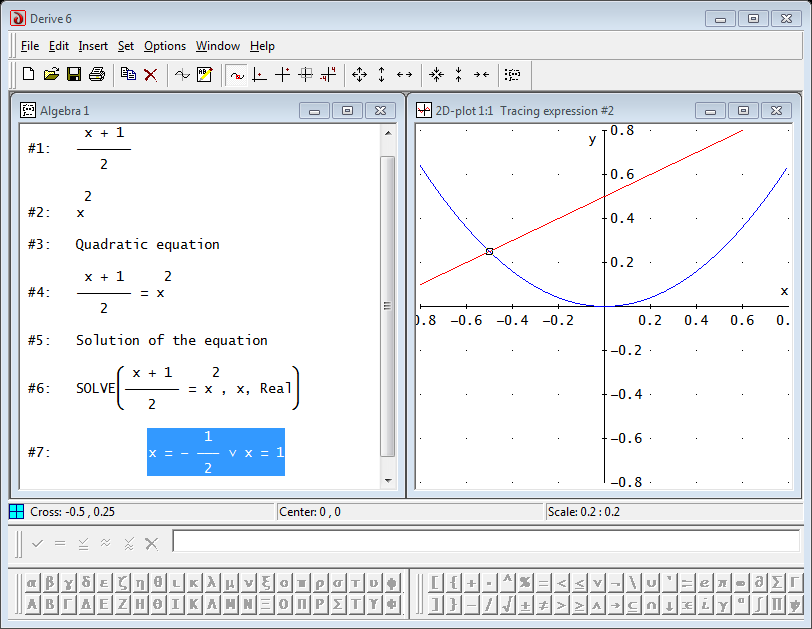
\includegraphics[width=0.8\textwidth]{img/introduction/trace_mode}
\caption{Graphic window in trace mode showing the point where two graphs intersect (that is one solution of the equation).}
\label{g:trace-mode}
\end{center}
\end{figure}


\subsubsection*{Centering the plot}
It is also possible to center the plot at the position of the cross with the button \button{Center on Cross} or at the origin of coordinates with the button \button{Center on Origin}.


\subsubsection*{2-dimensional graphical representations}
To represent a function or expression with 2 variables we have to select the expression and then the menu \menu{Window > New 3D-plot window}.
This will open a new graphic window with three Cartesian axes ($x$, $y$ and $z$).
Finally, to show the graph of the expression in the Cartesian space you have to select the menu \menu{Insert > Plot} or just click the corresponding button in the toolbar. 
Figure~\ref{g:3d-plot} shows an example of a 3-dimensional plot.

\begin{figure}[h!]
\begin{center}
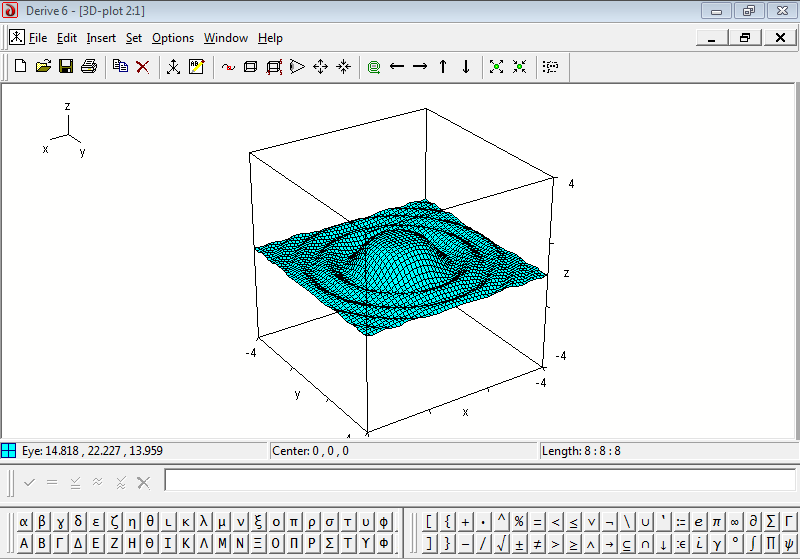
\includegraphics[scale=0.6]{img/introduction/3d-plot}
\caption{3-dimensional graphic window with the graph of a function.}
\label{g:3d-plot}
\end{center}
\end{figure}

Again it is possible to represent more than one function in the same 3-dimensional graphic window. 

Like for 2-dimensional graphic windows, there are several menus an buttons to change the aspect of the plot.

\subsubsection*{Changing the perspective of the plot}
One of the most interesting actions is changing the perspective of the plot with the menu \menu{Set > Eye Position}.
In the dialog shown you have to enter the coordinates of the observer eye and click the button \button{OK}.
It is also possible to change the perspective of the plot rotating the plot horizontally with the left/right arrow keys or vertically with the up/down arrow keys. 

\subsubsection*{Changing the resolution of the grid}
Derive plots the surfaces with a grid of small tiles. 
To change the resolution of the grid you can use the menu \menu{Edit > Plot}. 
In the dialog shown you can enter the number of vertical and horizontal panels.
The higher the number of panels the smoother the surface. 


\subsection*{File management}
The expressions and computations of an Algebra windows can be saved in a file.

\subsubsection*{Saving a file}
To save the content of an Algebra window in a file you can use the menu \menu{File > Save}.
In the dialog shown give a name to the file, select the folder where to save it and click the button \button{Save}.
Derive will put automatically extension \texttt{*.dfw} to the saved file. 
Once the file has been saved, its name will be shown in the title bar of the window. 


\subsubsection*{Opening a file}
To open a Derive file in an Algebra windows you can use the menu \menu{File > Open}.
In the dialog shown you only have to select the file that you want to open an click the button \button{Open}.
The selected file will be opened in a new Algebra window.


\subsubsection*{Opening and closing new Algebra windows}
Derive can manage more than one Algebra windows simultaneously. 
To open a new Algebra window you can use the menu \menu{File > New}. 
Derive works with each Algebra window independently.
That means that we can use the same names to refer to different constants or functions in different Algebra windows without interference. 

On the other side, to close an Algebra window you only have to use the menu 
\menu{File > Close}.


\subsubsection*{Printing}
To print the content of an Algebra window you can use the menu \menu{File > Print}.
However, before printing it is a good idea to preview the document with the menu 
\menu{File > Print Preview}. 
If everything is OK it is enough to click on the button \button{Print} to send the document to the printer. 
To change the margins and the orientation of the page you can use the menu \menu{File > Page Setup}.

Other options like the font, the header or the footer of the page can be set with the menu \menu{Options > Printing > Header and Footer}.


\subsubsection*{Getting help}
Like most Windows applications you can get help about the use of the program with the menu \menu{Help}.

% % Author: Alfredo Sánchez Alberca (asalber@ceu.es)
\chapter{Elementary functions}

% \section{Fundamentos teóricos}
% 
% En esta práctica se introducen los conceptos básicos sobre funciones reales de variable real, esto es, funciones
% \[f:\mathbb{R}\rightarrow \mathbb{R}.\]
% 
% \subsection{Dominio e imagen}
% 
% El \emph{Dominio} de la función $f$ es el conjunto de los números
% reales $x$ para los que existe $f(x)$ y se designa mediante $\dom
% f$.
% 
% La \emph{Imagen} de $f$ es el conjunto de los números reales $y$ para los que existe algún $x\in \mathbb{R}$ tal que $f(x)=y$, y se denota por $\im f$.
% 
% 
% \subsection{Signo y crecimiento}
% El \emph{signo} de la función es positivo $(+)$ en los valores de $x$ para los que $f(x)>0$ y negativo $(-)$ en los que $f(x)<0$. Los valores de $x$ en los que la función se anula se conocen como \emph{raíces} de la función.
% 
% Una función $f(x)$ es \emph{creciente} en un intervalo $I$ si $\forall\, x_1, x_2 \in I$ tales que $x_1<x_2$ se verifica que $f(x_1)\leq f(x_2)$.
% 
% Del mismo modo, se dice que una función $f(x)$ es \emph{decreciente} en un intervalo $I$ si $\forall\, x_1, x_2 \in I$ tales que $x_1<x_2$ se verifica que $f(x_1)\geq f(x_2)$. En la figura~\ref{g:crecimiento} se muestran estos conceptos.
% 
% \begin{figure}[h!]
% \centering \subfigure[Función creciente.] {\label{g:funcion_creciente}
% \scalebox{1}{\input{img/funciones_elementales/funcion_creciente}}}\qquad
% \subfigure[Función decreciente.]{\label{g:funcion_decreciente}
% \scalebox{1}{\input{img/funciones_elementales/funcion_decreciente}}}
% \caption{Crecimiento de una función.}
% \label{g:crecimiento}
% \end{figure}
% 
% 
% \subsection{Extremos Relativos}
% Una función $f(x)$ tiene un \emph{máximo relativo} en $x_0$ si existe un entorno $A$ de $x_0$ tal que $\forall x \in A$
% se verifica que $f(x)\leq f(x_0)$.
% 
% Una función $f(x)$ tiene un \emph{mínimo relativo} en $x_0$ si existe un entorno $A$ de $x_0$ tal que $\forall x\in A$
% se verifica que $f(x)\geq f(x_0)$.
% 
% Diremos que la función $f(x)$ tiene un \emph{extremo relativo} en un punto si tiene un \emph{máximo o mínimo relativo}
% en dicho punto. Estos conceptos se muestran en la figura~\ref{g:extremos}.
% 
% \begin{figure}[h!]
% \centering \subfigure[Máximo relativo.] {\label{g:maximo}
% \scalebox{1}{\input{img/funciones_elementales/maximo}}}\qquad
% \subfigure[Mínimo relativo.]{\label{g:minimo}
% \scalebox{1}{\input{img/funciones_elementales/minimo}}}
% \caption{Extremos relativos de una función.}
% \label{g:extremos}
% \end{figure}
% 
% Una función $f(x)$ está \emph{acotada superiormente} si $\exists K\in\mathbb{R}$ tal que $f(x)\leq K$ $\forall x \in \dom f$. Análogamente, se dice que una función $f(x)$ está \emph{acotada inferiormente} si $\exists K\in\mathbb{R}$ tal que $f(x)\geq K$ $\forall x \in \dom f$.
% 
% Una función $f(x)$ está \emph{acotada} si lo está superior e inferiormente, es decir si $\exists K\in\mathbb{R}$ tal que $|f(x)|\leq K$ $\forall x \in \dom f$.
% 
% 
% \subsection{Concavidad}
% 
% De forma intuitiva se puede decir que una función $f(x)$ es \emph{cóncava} en un intervalo $I$ si $\forall\, x_1, x_2
% \in I$, el segmento de extremos $(x_1,f(x_1))$ y $(x_2,f(x_2))$ queda por encima de la gráfica de $f$.
% 
% Análogamente se dirá que es \emph{convexa} si el segmento anterior queda por debajo de la gráfica de $f$.
% 
% Diremos que la función $f(x)$ tiene un \emph{punto de inflexión} en $x_0$ si en ese punto la función pasa de cóncava a
% convexa o de convexa a cóncava. Estos conceptos se ilustran en la figura~\ref{g:concavidad}.
% 
% \begin{figure}[h!]
% \centering \subfigure[Función cóncava.] {\label{g:funcion_concava_arriba}
% \scalebox{1}{\input{img/funciones_elementales/funcion_concava_arriba}}}\qquad
% \subfigure[Función convexa.]{\label{g:funcion_concava_abajo}
% \scalebox{1}{\input{img/funciones_elementales/funcion_concava_abajo}}}
% \caption{Concavidad de una función.}
% \label{g:concavidad}
% \end{figure}
% 
% \subsection{Asíntotas}
% 
% La recta $x=a$ es una \emph{asíntota vertical} de la función $f(x)$ si al menos uno de los límites laterales de $f(x)$ cuando $x$ tiende hacia $a$ es $+\infty$ o $-\infty$, es decir cuando se verifique alguna de las siguientes igualdades
% \[
% \ \lim_{x\rightarrow a^{+}}f(x)=\pm\infty   \quad \textrm{o} \quad
% \lim_{x\rightarrow a^{-}}f(x)=\pm\infty
% \]
% 
% La recta $y=b$ es una \emph{asíntota horizontal} de la función $f(x)$ si alguno de los límites de $f(x)$ cuando $x$ tiende hacia $+\infty$ o $-\infty$ es igual a $b$, es decir cuando se verifique
% \[
% \ \lim_{x\rightarrow -\infty }f(x)=b    \quad \textrm{o} \quad
% \ \lim_{x\rightarrow +\infty }f(x)=b
% \]
% 
% La recta $y=mx+n$ es una \emph{asíntota oblicua} de la función $f(x)$ si alguno de los límites de $f(x)-(mx+n)$ cuando $x$ tiende hacia $+\infty$ o $-\infty$ es igual a 0, es decir si
% 
% \[
% \ \lim_{x\rightarrow -\infty }{(f(x)-mx)}=n    \quad \textrm{o} \quad
% \ \lim_{x\rightarrow +\infty }{(f(x)-mx)}=n
% \]
% 
% En la figura~\ref{g:asintotas} se muestran los distintos tipos de asíntotas.
% 
% \begin{figure}[h!]
% \centering \subfigure[Asíntota horizontal y vertical.] {\label{g:asintotahorizontalyvertical}
% \scalebox{1}{\input{img/funciones_elementales/asintota_vertical_horizontal}}}\qquad\qquad
% \subfigure[Asíntota vertical y oblicua.]{\label{g:asintotaoblicua}
% \scalebox{1}{\input{img/funciones_elementales/asintota_oblicua}}}
% \caption{Tipos de asíntotas de una función.}
% \label{g:asintotas}
% \end{figure}
% 
% 
% \subsection{Periodicidad}
% Una función $f(x)$ es \emph{periódica} si existe $h\in\mathbb{R^{+}}$ tal que \[f(x+h)=f(x)\  \forall x\in \dom f\] siendo el período $T$ de la función, el menor valor $h$ que verifique la igualdad anterior.
% 
% En una función periódica, por ejemplo $f(x)=A\sin(wt)$, se denomina \emph{amplitud} al valor de $A$, y es la mitad de la diferencia entre los valores máximos y mínimos de la función. En la figura~\ref{g:periodoyamplitud} se ilustran estos conceptos.
% 
% \begin{figure}[h!]
% \centering
% \scalebox{0.8}{\input{img/funciones_elementales/funcion_periodica}}
% \caption{Periodo y amplitud de una función periódica.}
% \label{g:periodoyamplitud}
% \end{figure}
% 
% \clearpage
% \newpage

\section{Solved exercises}

\begin{enumerate}[leftmargin=*]
\item Consider the function
\[
f(t)=\frac{t^4+19t^2-5}{t^4+9t^2-10}.
\]
 
\begin{enumerate}
\item Plot the graph of the function. 
\begin{indication}
\begin{enumerate}
\item Enter the expression of the function and select it. 
\item Select the menu \menu{Window > New 2D-plot Window}.
\item In the graphic window click the button \button{Plot}.
\end{enumerate}
\end{indication}

\item Looking at the graph of the function determine:
\begin{enumerate}
\item Domain.
\begin{indication}
Look at the values of $x$ where the function does exists, that is, where there is graph.
\end{indication}

\item  Image.
\begin{indication}
Look at the values of $y$ that are output of the function, that is, where there is graph. 
\end{indication}

\item  Asymptotes.
\begin{indication}
Look at the lines (horizontal, vertical or oblique) where the graph approaches (the distance between the graph and the line tends to zero as they tend to infinity).
\end{indication}

\item  Zeros.
\begin{indication}
Look at the values of $x$  where the graph cuts the horizontal axis. 
\end{indication}

\item Sign.
\begin{indication}
Look at the values of $x$ where the graph is over the horizontal axis (positive) and where it is under the horizontal axis (negative).
\end{indication}

\item Continuity
\begin{indication}
Look at the values of $x$ where you can trace the graph without lifting your hand. 
\end{indication}

\item Increasing and decreasing.
\begin{indication}
Look at the values of $x$ where $y$ increases when $x$ increases (increasing) and the values where $y$ decreases when $x$ increases (decreasing).
\end{indication}

\item Concavity
\begin{indication}
Look at the values of $x$ where the curvature of the graph is up $\cup$ (concave up or convex) and where the curvature is down $\cap$ (concave down or simply concave).
\end{indication}

\item Relative extrema.
\begin{indication}
Look at the values of $x$ where the graph has a peak (relative maximum) and where the graph has a valley (relative minimum).
\end{indication}

\item Inflection points.
\begin{indication}
Look at the values of $x$ where the curvature changes continuously. 
\end{indication}
\end{enumerate}
\end{enumerate}


\item Plot in the same graphic window the graphs of the functions $2^x$, $e^x$, $0.7^x$, $0.5^x$. 
Looking at the graphs of the functions, determine which ones are increasing and which ones are decreasing. 

\begin{indication}
Open a new graphic window with the menu \menu{Window > New 2d-plot Window} and select the menu \menu{Window -> Tile Vertically} to see the Algebra and the graphic windows at the same time. 

For every function repeat the following steps:
\begin{enumerate}
\item Enter the expression of the function in the Algebra window and select it. 
\item Click the button \button{Plot} in the graphic window.
\item Click at some point near the graph and select the menu \menu{Insert > Annotation}. 
In the dialog shown enter the name of the function and click the button \button{OK}.
\end{enumerate}
\end{indication}

Can you deduce for what values of $a$ the function $a^x$ is increasing and for what values it is decreasing?


\item Plot in the same graphic window the graphs of the following functions and determine their periods and amplitudes. 
\begin{enumerate}
\item $\sin(x)$, $\sin(x)+2$, $\sin(x+2)$.
\item $\sin(2x)$, $2\sin(x)$, $\sin(x/2)$.
\begin{indication}
Open a new graphic window with the menu \menu{Window > New 2d-plot Window} and select the menu \menu{Window -> Tile Vertically} to see the Algebra and the graphic windows at the same time. 
For every function repeat the following steps:
\begin{enumerate}
\item Enter the expression of the function in the Algebra window and select it. 
\item Click the button \button{Plot} in the graphic window.
\item Click at some point near the graph and select the menu \menu{Insert > Annotation}. 
In the dialog shown enter the name of the function and click the button \button{OK}.
\end{enumerate}
For the period look at the length of the smaller interval in the horizontal axis where the graph is repeated. 

For the amplitude look at the distance between the maximum and the minimum and divide it by two.
\end{indication}
\end{enumerate}


\item Plot the piecewise function 
\[
f(x)=
\begin{cases}
-2x & \mbox{if $x\leq0$;} \\
x^2 & \mbox{if $x>0$.}
\end{cases}
\]

\begin{indication}
To represent a piecewise function Derive uses the function \command{CHI}.
The syntax for this function is \command{CHI(a,x,b)}, where \command{a} and \command{b} are the lower and upper limits where a subfunction is defined and \command{x} is the variable of the function. 
This defines the function 
\[
\operatorname{CHI} (a,x,b) = 
\begin{cases}
0 & \mbox{if $x<a$} \\
1 & \mbox{if $a\leq x \leq b$} \\
0 & \mbox{if $x>b$}
 \end{cases}
\]

According to this, to enter the piecewise function we have to write  
\[
\command{-2x CHI(-inf,x,0) + x\^{}2 CHI(0,x,inf)}
\]
\end{indication}
\end{enumerate}


\section{Proposed exercises}
\begin{enumerate}[leftmargin=*]
\item Plot the graphs of the following functions and determine their domains looking at their graphs.  

\begin{enumerate}
\item $f(x)=\dfrac{x^2+x+1}{x^3-x}$
\item $g(x)=\sqrt{x^4-1}$.
\item $h(x)=\cos\left(\frac{x+3}{x^2+1}\right)$.
\item $l(x)=\arcsin\left(\frac{x}{1+x}\right)$.
\end{enumerate}

\item Consider the function
\[
f(x)=\frac{x^3+x+2}{5x^3-9x^2-4x+4}.
\]

Plot the function and determine looking at its graph:
\begin{enumerate}
\item Domain
\item Image
\item Asymptotes
\item Zeros
\item Sign
\item Continuity
\item Increasing and decreasing
\item Concavity
\item Relative extrema
\item Inflection points
\end{enumerate}

\item Plot in the same graphic window the graphs of the functions $\log_{10}x$, $\log_{2}x$, $\log x$, $\log_{0.5}x$.
\begin{enumerate}
\item Looking at their graphs determine which funtions are increasing and which ones are decreasing.
\item Deduce for what values of $a$ the function $\log_ax$ is increasing and for what values it is decreasing?
\end{enumerate}

\item Plot the following functions and complete the following sentences with the word equal or the number of times that is lower or greater in any case.
\begin{enumerate}
\item The function $\cos(2x)$ has a period ............ than the function $\cos{x}$.
\item The function $\cos(2x)$ has an amplitude ............ than the function $\cos{x}$.
\item The function $\cos(x/2)$ has period ............ than the function $\cos(3x)$.
\item The function $\cos(x/2)$ has an amplitude ............ than the function $\cos(3x)$.
\item The function $3\cos(2x)$ has a period ............ than the function $\cos(x/2)$.
\item The function $3\cos(2x)$ has an amplitude ............ than the function $\cos(x/2)$.
\end{enumerate}

\item Find the solutions of the equation $e^{-1/x}=\dfrac{1}{x}$  graphically.

\item Plot the graph of the function
\[
f(x)=
\begin{cases}
x^3 & \mbox{if $x<0$} \\
e^x-1 & \mbox{if $x\geq0$}
\end{cases}
\]
\end{enumerate}

% Author: Alfredo Sánchez Alberca (asalber@ceu.es)
\chapter{Limits and continuity}

% \section{Fundamentos teóricos}
% En esta práctica se introducen los conceptos de límite y continuidad de una función real, ambos muy relacionados.
% 
% \subsection{Límite de una función en un punto}
% El concepto de límite está muy relacionado con el de proximidad y tendencia de una serie de valores. De manera informal, diremos que $l\in \mathbb{R}$ es el \emph{límite} de una función $f(x)$ en un punto $a\in \mathbb{R}$, si $f(x)$ tiende o se aproxima cada vez más a $l$, a medida que $x$ se aproxima a $a$, y se escribe
% \[ \lim_{x\rightarrow a} f(x)=l.\]
% 
% Si lo que nos interesa es la tendencia de $f(x)$ cuando nos aproximamos al punto $a$ sólo por un lado, hablamos de \emph{límites laterales}. Diremos que $l$ es el \emph{límite por la izquierda} de una función $f(x)$ en un punto $a$, si $f(x)$ tiende o se aproxima cada vez más a $l$, a medida que $x$ se aproxima a $a$ por la izquierda, es decir con valores $x<a$, y se denota por
% \[ \lim_{x\rightarrow a^-} f(x)=l.\]
% Del mismo modo, diremos que $l$ es el \emph{límite por la derecha} de una función $f(x)$ en un punto $a$, si $f(x)$ tiende o se aproxima cada vez más a $l$, a medida que $x$ se aproxima a $a$ por la derecha, es decir con valores $x>a$, y se denota por
% \[ \lim_{x\rightarrow a^+} f(x)=l.\]
% 
% Por supuesto, para que exista el límite global de la función $f(x)$ en el punto $a$, debe existir tanto el límite por la izquierda, como el límite por la derecha, y ser iguales, es decir
% \[
% \left.
% \begin{array}{l}
% \displaystyle \lim_{x\rightarrow a^-} f(x)=l\\
% \displaystyle \lim_{x\rightarrow a^+} f(x)=l
% \end{array}
% \right\}
% \Longrightarrow
% \lim_{x\rightarrow a} f(x)=l.
% \]
% 
% \subsection{Álgebra de límites}
% Para el cálculo práctico de límites, se utiliza el siguiente
% teorema, conocido como Teorema de \emph{Álgebra de Límites}.
% 
% Dadas dos funciones $f(x)$ y $g(x)$, tales que $\lim_{x\rightarrow
% a}f(x)=l_1$ y $\lim_{x\rightarrow a}g(x)=l_2$, entonces se cumple
% que:
% \begin{enumerate}
% \item $\displaystyle \lim_{x\rightarrow a}(f(x)\pm g(x))=l_1\pm l_2$.
% \item $\displaystyle \lim_{x\rightarrow a}(f(x)\cdot g(x))=l_1\cdot l_2$.
% \item $\displaystyle \lim_{x\rightarrow a}\dfrac{f(x)}{g(x)}=\dfrac{l_1}{l_2}$ si $l_2\neq 0$.
% \end{enumerate}
% 
% \subsection{Asíntotas}
% Como interpretación geométrica de los límites, definiremos rectas
% particulares a las que tiende (se ``pega") la gráfica de una función
% cuando la variable tiende a un cierto valor, finito o infinito.
% \subsubsection*{Asíntotas verticales}
% La recta $x=a$ es una \emph{Asíntota Vertical} de la función $f(x)$
% si al menos uno de los límites laterales de $f$ en $a$ es $+\infty$
% ó $+\infty$. Es decir:
% 
% \[
% \mathop {\lim }\limits_{x \to a} f(x) =  \pm \infty
% \]
% 
% \subsubsection*{Asíntotas Horizontales}
% La recta $y=b$ es una \emph{Asíntota Horizontal} de la función
% $f(x)$ si se cumple:
% \[
% \mathop {\lim }\limits_{x \to  + \infty } f(x) = b\quad
% \text{ó}\quad\mathop {\lim }\limits_{x \to  - \infty } f(x) = b
% \]
% 
% 
% \subsubsection*{Asíntotas Oblicuas}
% 
% La recta $y=mx+n$, donde $m\neq0$, es \emph{Asíntota Oblicua} de la
% función $f(x)$ si:
% 
% 
% \[
% \mathop {\lim }\limits_{x \to  + \infty } \left[ {f(x) - \left( {mx
% + n} \right)} \right] = 0\quad\text{ó}\quad\mathop {\lim }\limits_{x
% \to - \infty } \left[ {f(x) - \left( {mx + n} \right)} \right] = 0
% \]
% 
% 
% La determinación práctica de $m$ y $n$ se realiza del siguiente
% modo:
% 
% \[
% m = \mathop {\lim }\limits_{x \to  + \infty } \frac{{f(x)}} {x}
% \]
% 
% \[
% n = \mathop {\lim }\limits_{x \to  + \infty } \left[ {f(x) - mx}
% \right]
% \]
% o bien lo mismo con los límites en $-\infty$:
% \[
% m = \mathop {\lim }\limits_{x \to  - \infty } \frac{{f(x)}} {x}
% \]
% 
% \[
% n = \mathop {\lim }\limits_{x \to  - \infty } \left[ {f(x) - mx}
% \right]
% \]
% 
% En cualquiera de los casos, si obtenemos un valor real para $m$ (no
% puede ser ni $+\infty$ ni $-\infty$) distinto de $0$, procedemos
% después a calcular $n$, que también debe ser real (sí que puede ser
% $0$).
% 
% Si $m=\pm\infty$ entonces la función crece (decrece) más deprisa que
% cualquier recta, y si $m=0$ la función crece (decrece) más despacio
% que cualquier recta, y en cualquiera de los dos casos decimos que la
% función tiene una \emph{Rama Parabólica}.
% 
% \subsection{Continuidad de una función en un punto}
% Diremos que una función $f(x)$ es continua en un punto $a\in
% \mathbb{R}$, si se cumple
% \[ \lim_{x\rightarrow a}f(x)=f(a),\]
% donde $f(a)\in \mathbb{R}$.
% 
% La definición anterior implica a su vez que se cumplan estas tres
% condiciones:
% 
% \begin{itemize}
% 
% \item Existe el límite de $f$ en $x=a$.
% 
% \item La función está definida en $x=a$; es decir, existe $f(a)$.
% 
% \item Los dos valores anteriores coinciden.
% 
% \end{itemize}
% 
% Si la función $f$ no es continua en $x=a$, diremos que es
% \emph{discontinua} en el punto $a$, o bien que $f$ tiene una
% \emph{discontinuidad} en $a$.
% 
% Intuitivamente, una función es continua cuando puede dibujarse su
% gráfica sin levantar el lápiz.
% 
% \subsubsection*{Continuidad lateral en un punto}
% 
% Si nos restringimos a los valores que toma una función a la derecha
% de un punto $x=a$, o a la izquierda, se habla de continuidad por la
% derecha o por la izquierda según la siguiente definición.
% 
% Una función es \emph{continua por la derecha} en un punto $x=a$, y
% lo notaremos como $f$ continua en $a^+$, si existe el límite por la
% derecha en dicho punto y coincide con el valor de la función en el
% mismo:
% \[
% \mathop {\lim }\limits_{x \to a^ +  } f\left( x \right) = f\left( a
% \right)
% \]
% 
% De igual manera, la función es \emph{continua por la izquierda} en
% un punto $x=a$, y lo notaremos como $f$ continua en $a^-$, si existe
% el límite por la izquierda en dicho punto y coincide con el valor de
% la función en el mismo:
% 
% \[
% \mathop {\lim }\limits_{x \to a^ -  } f\left( x \right) = f\left( a
% \right)
% \]
% 
% 
% \subsubsection*{Propiedades de la continuidad en un punto}
% 
% Como consecuencia de la definición de continuidad en un punto,
% podrían demostrarse toda una serie de teoremas, algunos de ellos
% especialmente importantes.
% 
% \begin{itemize}
% 
% \item \textbf{Álgebra de funciones continuas}.
% Si $f$ y $g$ son funciones continuas en $x=a$, entonces $f\pm g$ y
% $f\cdot g$ son también continuas en $x=a$. Si además $g(a)\neq 0$,
% entonces $f/g$ también es continua en $x=a$.
% 
% \item \textbf{Continuidad de funciones compuestas}. Si $f$ es continua en
% $x=a$ y $g$ es continua en $b=f(a)$, entonces la función compuesta
% $g\circ f$ es continua en $x=a$.
% 
% \item \textbf{Continuidad y cálculo de límites}. Sean $f$ y $g$ dos
% funciones tales que existe $\mathop {\lim }\limits_{x \to a} f(x) =
% l$ $\in \mathbb{R}$ y $g$ es una función continua en $l$. Entonces:
% 
% \[
% \mathop {\lim }\limits_{x \to a} g\left( {f\left( x \right)} \right)
% = g\left( l \right)
% \]
% 
% \end{itemize}
% 
% \subsubsection*{Tipos de discontinuidades}
% Puesto que la condición de continuidad puede no satisfacerse por
% distintos motivos, existen distintos tipos de discontinuidades:
% 
% 
% \begin{itemize}
% \item \textbf{Discontinuidad evitable}. Se dice que $f(x)$ tiene una \emph{discontinuidad evitable} en el punto $a$, si existe el límite de la función  pero no coincide con el valor de la función en el punto (bien porque sea diferente, bien por que la función no esté definida en dicho punto), es decir
% \[\lim_{x\rightarrow a}f(x)=l\neq f(a).\]
% 
% \item \textbf{Discontinuidad de salto}. Se dice que $f(x)$ tiene una \emph{discontinuidad de salto} en el punto $a$, si existe el límite de la función por la izquierda  y por la derecha pero son diferentes, es decir,
% \[
% \lim_{x\rightarrow a^-}f(x)=l_1\neq l_2=\lim_{x\rightarrow a^+}f(x).
% \]
% A la diferencia entre ambos límites $l_1-l_2$, se le llama
% \emph{amplitud del salto}.
% 
% \item \textbf{Discontinuidad esencial}. Se dice que $f(x)$ tiene una \emph{discontinuidad esencial} en el punto $a$, si no existe alguno de los límites laterales de la función.
% \end{itemize}
% 
% \newpage

\section{Solved exercises}
\begin{enumerate}[leftmargin=*]
\item Given the function
\[
f(x)=\left( 1+\frac 2x\right) ^{x/2},
\]

plot its graph and compute the following limits:

\begin{multicols}{2}
\begin{enumerate}
\item  $\lim\limits_{x\rightarrow -\,\infty }\ f(x)$
\item  $\lim\limits_{x\rightarrow +\,\infty }\ f(x)$
\item  $\lim\limits_{x\rightarrow -\,2^{-}}\ f(x)$
\item  $\lim\limits_{x\rightarrow -\,2^{+}}\ f(x)$
\item  $\lim\limits_{x\rightarrow 2}\ f(x)$
\item  $\lim\limits_{x\rightarrow 0}\ f(x)$
\end{enumerate}
\end{multicols}

\begin{indication}
\begin{enumerate}
\item Enter the expression of the function in the Algebra window and select it.
\item Open a new graphic window with the menu \menu{Window > New 2d-plot Window} and select the menu \menu{Window -> Tile Vertically} to see the Algebra and the graphic windows at the same time.  
\item Click the button \button{Plot} in the graphic window.
\item For computing every limit repeat the following steps
\begin{enumerate}
\item Select the function in the Algebra window.
\item Select the menu \menu{Calculus > Limit} or click the button \button{Limit}.
\item In the dialog shown enter the point of the limit in the field \field{Limit Point}, select the corresponding option from the list \field{Approach From} (\option{Left} for a one-sided limit from the left, \option{Right} for a one-sided limit from the right, and \option{Both} for a global or two-sided limit) and click the button \button{Simplify}.
\item Look at the graph and check if the result of the limit makes sense. 
\end{enumerate}
\end{enumerate}
\end{indication}


\item Given the function 
\[
f(x)=
\begin{cases}
\dfrac{x}{x-2} & \mbox{if $x\leq 0$;}\\
\dfrac{x^2}{2x-6} & \mbox{if $x>0$;}
\end{cases}
\]
\begin{enumerate}
\item Plot the graph and determine graphically if there are asymptotes. 
\begin{indication}
\begin{enumerate}
\item Enter the expression \command{f(x) := x/(x-2) CHI(-inf,x,0) + x\^{}2/(2x-6) CHI(0,x,inf)} to define the function in the Algebra window and select the function.
\item Open a new graphic window with the menu \menu{Window > New 2d-plot Window} and select the menu \menu{Window -> Tile Vertically} to see the Algebra and the graphic windows at the same time.  
\item Click the button \button{Plot} in the graphic window.
\end{enumerate}
\end{indication}

\item Compute the vertical asymptotes and plot them if any. 
\begin{indication}
The only point where the function is not defined is $x=3$.
Thus to check if there is a vertical asymptote at this point we have to compute the limit at this point. 
\begin{enumerate}
\item Select the name of function in the Algebra window.
\item Select the menu \menu{Calculus > Limit} or click the button \button{Limit}.
\item In the dialog shown enter 3 in the field \field{Limit Point}, select \command{Left} from the list \field{Approach From} and click the button \button{Simplify}. 
\item Repeat the three previous steps but selecting \command{Right} from the list \field{Approach From}.
\item Look at the graph and check if the results of the limits make sense. 
\end{enumerate}
There is a vertical asymptote $x=3$ if some of the limits is infinite.
In that case enter the expression of the asymptote in the Algebra window and click the button \button{Plot} in the graphic window.
\end{indication}

\item Compute the horizontal asymptotes and plot them if any.
\begin{indication}
To check if there is an horizontal asymptote we have to compute the limits at infinity.
\begin{enumerate}
\item Select the name of function in the Algebra window.
\item Select the menu \menu{Calculus > Limit} or click the button \button{Limit}.
\item In the dialog shown enter \command{-inf} in the field \field{Limit Point} and click the button \button{Simplify}. 
\item Repeat the two previous steps but selecting entering \command{inf} in the field \field{Limit Point}.
\item Look at the graph and check if the results of the limits make sense. 
\end{enumerate}
There is an horizontal asymptote $y=a$ if some of the limits is $a$.
In that case enter the expression of the asymptote in the Algebra window and click the button \button{Plot} in the graphic window. 
\end{indication}

\item Compute the oblique asymptotes and plot them if any.
\begin{indication}
To check if there is an oblique asymptote we have to compute the limits at infinity of the function divided by $x$.
To check if there is an oblique asymptote at $-\infty$, do the following steps:
\begin{enumerate}
\item Enter the expression \command{f(x)/x} in the Algebra window and select it.
\item Select the menu \menu{Calculus > Limit} or click the button \button{Limit}.
\item In the dialog shown enter \command{-inf} in the field \field{Limit Point} and click the button \button{Simplify}. 
\end{enumerate}
There is an oblique asymptote $y=ax+b$ if some of the limits is $a$.
In that case, $a$ is the slope of the asymptote. 
To compute the independent term we have to compute the limits at infinity of the function minus $ax$.
\begin{enumerate}
\item Enter the expression \command{f(x)-ax}, where \command{a} is the value of the previous limit, in the Algebra window and select it.
\item Select the menu \menu{Calculus > Limit} or click the button \button{Limit}.
\item In the dialog shown enter \command{-inf} in the field \field{Limit Point} and click the button \button{Simplify}. 
\end{enumerate}
The independent term of the oblique asymptote is the result of this limit.

To check if there is an oblique asymptote at $\infty$, repeat all the steps but entering \command{inf} in the field \field{Limit Point}.
 
If there is some oblique asymptote enter the expression of the asymptote in the Algebra window and click the button \button{Plot} in the graphic window.
\end{indication}
\end{enumerate}

\item For the following functions determine the type of discontinuity at the points given.
\begin{enumerate}
\item $f(x)=\dfrac{\sin x}{x}$ at $x=0$.
\item $g(x)=\dfrac{1}{2^{1/x}}$ at $x=0$.
\item $h(x)=\dfrac{1}{1+e^{\frac{1}{1-x}}}$ at $x=1$.
\end{enumerate}

\begin{indication}
For every function repeat the following steps:
\begin{enumerate}
\item Enter the expression of the function in the Algebra window and select it.
\item Open a new graphic window with the menu \menu{Window > New 2d-plot Window} and select the menu \menu{Window -> Tile Vertically} to see the Algebra and the graphic windows at the same time.  
\item Click the button \button{Plot} in the graphic window.
\item Select the function in the Algebra window.
\item Select the menu \menu{Calculus > Limit} or click the button \button{Limit}.
\item In the dialog shown enter the given point in the field \field{Limit Point}, select \command{Left} from the list \field{Approach From} and click the button \button{Simplify}. 
\item Repeat the three previous steps but selecting \command{Right} from the list \field{Approach From}.
\end{enumerate}
If both limits exist and are the same, then there is a \emph{removable discontinuity}. 
If both limits exist but are different, then there is a \emph{jump discontinuity}.
If some of the limits doesn't exist or is infinite, then there is an \emph{essential discontinuity}.  
\end{indication}


\item Determine the points where the following function has a discontinuity and classify it.
\[
f(x)=
\begin{cases}
\dfrac{x+1}{x^2-1}, & \mbox{if $x<0$;} \\
\dfrac{1}{e^{1/(x^2-1)}}, & \mbox{if $x\geq 0$.}
\end{cases}
\]

\begin{indication}
\begin{enumerate}
\item Enter the expression \command{f(x) := (x+1)/(x\^{}2-1) CHI(-inf,x,0) + 1/exp(1/(x\^{}2-1)) CHI(0,x,inf)} to define the function in the Algebra window and select the function.
\item Open a new graphic window with the menu \menu{Window > New 2d-plot Window} and select the menu \menu{Window -> Tile Vertically} to see the Algebra and the graphic windows at the same time.  
\item Click the button \button{Plot} in the graphic window.
\end{enumerate}
The function is not defined in $x=-1$ and $x=1$, so there is a discontinuity at each of these points. 
As the functions is piecewise, also we have to study the points where the expression of the function changes, that is, at $x=0$.
To classify the type of discontinuity for each of these points, repeat the following steps:
\begin{enumerate}
\item Select the function in the Algebra window.
\item Select the menu \menu{Calculus > Limit} or click the button \button{Limit}.
\item In the dialog shown enter the given point in the field \field{Limit Point}, select \command{Left} from the list \field{Approach From} and click the button \button{Simplify}. 
\item Repeat the three previous steps but selecting \command{Right} from the list \field{Approach From}.
\end{enumerate}
If both limits exist and are the same, then there is a \emph{removable discontinuity}. 
If both limits exist but are different, then there is a \emph{jump discontinuity}.
If some of the limits doesn't exist or is infinite, then there is an \emph{essential discontinuity}.  
\end{indication}
\end{enumerate}


\section{Proposed exercises}
\begin{enumerate}[leftmargin=*]
\item Compute the following limits:
\begin{multicols}{2}
\begin{enumerate}
\item $\displaystyle \lim_{x\rightarrow 1}\dfrac{x^3-3x+2}{x^4-4x+3}$.
\item $\displaystyle \lim_{x\rightarrow a}\dfrac{\sin x-\sin a}{x-a}$.
\item $\displaystyle \lim_{x\rightarrow\infty}\dfrac{x^2-3x+2}{e^{2x}}$.
\item $\displaystyle \lim_{x\rightarrow\infty}\dfrac{\log(x^2-1)}{x+2}$.
\item $\displaystyle \lim_{x\rightarrow 1}\dfrac{\log(1/x)}{\tan(x+\dfrac{\pi}{2})}$.
\item $\displaystyle \lim_{x\rightarrow a}\dfrac{x^n-a^n}{x-a}\quad n\in \mathbb{N}$.
\item $\displaystyle \lim_{x\rightarrow 1}\dfrac{\sqrt[n]{x}-1}{\sqrt[m]{x}-1}\quad n,m \in \mathbb{Z}$.
\item $\displaystyle \lim_{x\rightarrow 0}\dfrac{\tan x-\sin x}{x^3}$.
\item $\displaystyle \lim_{x\rightarrow \pi/4}\dfrac{\sin x-\cos x}{1-\tan x}$.
\item $\displaystyle \lim_{x\rightarrow 0}x^2e^{1/x^2}$.
\item $\displaystyle \lim_{x\rightarrow \infty}\left(1+\dfrac{a}{x}\right)^x$.
\item $\displaystyle \lim_{x\rightarrow 0}\left(\dfrac{1}{x}\right)^{\tan x}$.
\item $\displaystyle \lim_{x\rightarrow 0}(\cos x)^{1/\mbox{\footnotesize sen}\, x}$.
\item $\displaystyle \lim_{x\rightarrow 0}\dfrac{6}{4+e^{-1/x}}$.
\item $\displaystyle \lim_{x\rightarrow \infty}\left(\sqrt{x^2+x+1}-\sqrt{x^2-2x-1}\right)$.
\end{enumerate}
\end{multicols}

\item Given the function 
\[
f(x) = 
\begin{cases}
\dfrac{x^2+1}{x+3} & \mbox{if $x<0$}; \\
\dfrac{1}{e^{1/(x^2-1)}} & \mbox{if $x\geq 0$;}
\end{cases} 
\]
compute its asymptotes.

\item The following functions are not defined at $x=0$.
Determine, when possible, the value that should take the function at that point to be continuous. 
\begin{multicols}{2}
\begin{enumerate}
\item $f(x)=\dfrac{(1+x)^n-1}{x}$.
\item $h(x)=\dfrac{e^x-e^{-x}}{x}$.
\item $j(x)=\dfrac{\log(1+x)-\log(1-x)}{x}$.
\item $k(x)=x^2\sin\dfrac{1}{x}$.
\end{enumerate}
\end{multicols}

\end{enumerate}

% % Author: Alfredo Sánchez Alberca (asalber@ceu.es)
\chapter{Derivatives of functions of one variable}

% \section{Fundamentos teóricos}
% El concepto de derivada es uno de los más importantes del Cálculo
% pues resulta de gran utilidad en el estudio de funciones y tiene
% multitud de aplicaciones. En esta práctica introducimos este
% concepto y presentamos algunas de sus aplicaciones, tanto en
% funciones de una como de varias variables.
% 
% \subsection{Tasas de variación media e instantánea. La derivada}
% Cuando queremos conocer la variación que experimenta una función
% real $f(x)$ en un intervalo $[a,b]$, se calcula la diferencia
% $f(b)-f(a)$ que se conoce como \emph{incremento} de $f$, y se nota
% $\Delta f[a,b]$, aunque, a veces, simplemente se escribe $\Delta f$.
% 
% En muchas otras ocasiones veces resulta importante comparar la
% variación que experimenta la función $f$ con relación a la variación
% que experimenta su argumento $x$ en un intervalo $[a,b]$. Si tenemos
% en cuenta que $b=a+\Delta x$, esto viene dado por la \emph{tasa de
% variación media}, que se define como:
% 
% \[
% \textrm{TVM} f[a,b]=\textrm{TVM} f[a,a+\Delta x]=\frac{\Delta
% f}{\Delta x}=\frac{f(b)-f(a)}{b-a}=\frac{f(a+\Delta x )-f(a)}{\Delta
% x}.
% \]
% 
% También resulta muy común llamar a $\Delta x$ con la letra $h$, por
% lo que la expresión anterior queda de la forma:
% 
% \[
% \textrm{TVM} f[a,b]=\textrm{TVM} f[a,a+h]=\frac{\Delta f}{\Delta
% x}=\frac{f(a+h)-f(a)}{h}.
% \]
% 
% Desde el punto de vista geométrico, la tasa de variación media de
% $f$ en el intervalo $[a , a+\Delta x]$ es la pendiente de la recta
% secante a $f$ en los puntos $(a , f(a))$ y $(a+\Delta x, f(a+\Delta
% x))$, tal y como se muestra en la figura~\ref{g:secante}.
% 
% \begin{figure}[h!]
% \begin{center}
% \scalebox{1}{\input{img/derivadas/secante}}
% \caption{La tasa de variación media como la pendiente de la recta
% secante a una función en dos puntos.} \label{g:secante}
% \end{center}
% \end{figure}
% 
% 
% Y, a veces, incluso más importante que la tasa de variación media,
% es estudiar la tasa de variación que experimenta la función, no en
% un intervalo, sino en un punto, tomando para ello límites cuando el
% incremento en la variable independiente tiende 0. Definimos la tasa
% de variación de una función en un punto $a$, o también tasa de
% variación instantánea, a partir de la tasa de variación media de la
% función en el intervalo $[a,a+\Delta x]$. Dicha tasa, si existe,
% recibe el nombre de \emph{derivada} de la función real $f(x)$ en un
% punto $a\in \mathbb{R}$, y se nota como $f'(a)$, o bien
% $\dfrac{df}{dx}(a)$:
% 
% \[
% f'(a)=\dfrac{df}{dx}(a)= \lim_{\Delta x\rightarrow 0}\frac{\Delta
% f}{\Delta x}=\lim_{\Delta x\rightarrow 0}\frac{f(a+\Delta
% x)-f(a)}{\Delta x}=\lim_{h\rightarrow 0}\frac{f(a+h)-f(a)}{h}.
% \]
% 
% Cuando este límite existe, se dice que la función $f$ es
% \emph{derivable} o \emph{diferenciable} en el punto $a$.
% 
% Geométricamente, $f'(a)$ es la pendiente de la recta tangente a la
% curva de $f(x)$ en el punto $(a,f(a))$, tal y como se aprecia en la
% figura~\ref{g:tangente}.
% 
% \begin{figure}[h!]
% \begin{center}
% \scalebox{1}{\input{img/derivadas/tangente}}
% \caption{La derivada como la pendiente de la recta tangente a una
% función en un punto.} \label{g:tangente}
% \end{center}
% \end{figure}
% 
% \subsubsection*{Recta tangente y normal a una función en un punto}
% De la gráfica anterior, fácilmente se deduce que la ecuación de la
% recta tangente a una función $f(x)$ en el punto $(a,f(a))$ es:
% \[
% y=f(a)+f'(a)(x-a).
% \]
% 
% Y teniendo en cuenta que la pendiente de la recta normal (recta
% perpendicular a la recta tangente) es la inversa cambiada de signo,
% la ecuación de la recta normal a $f(x)$ en el punto $(a,f(a))$ es:
% \[
% y=f(a)-\frac{1}{f'(a)}(x-a).
% \]
% 
% \subsection{Función derivada y derivadas sucesivas}
% 
% El límite que nos sirve para calcular la derivada de una función en
% un punto, define una nueva función $f'$ cuyo dominio está formado
% por los puntos en los que $f$ es diferenciable. La función $f'(x)$,
% o también $\dfrac{df}{dx}$, se llama \emph{primera derivada} de $f$.
% 
% Puesto que $f'$ es una función, puede derivarse a su vez, y la
% primera derivada de $f'$ se conoce como segunda derivada de $f$, y
% se nota $f''(x)$ o $\dfrac{d^2f}{dx^2}$. Análogamente, la
% \emph{$n$-ésima derivada} de $f$, designada por $f^{(n}$ o
% $\dfrac{d^nf}{dx^n}$, es la primera derivada de $f^{(n-1}$, para
% $n=2,3,\ldots$, es decir
% \[
% \frac{d^nf}{dx^n}=\frac{d}{dx}\left(\frac{d^{n-1}f}{dx^{n-1}}\right)\
% n=2,3,\ldots
% \]
% 
% 
% \subsection{Estudio del crecimiento de una función}
% Una función $f(x)$ es \emph{creciente} en un intervalo $I$ si
% $\forall\, x_1, x_2 \in I$ tales que $x_1<x_2$ se verifica que
% $f(x_1)\leq f(x_2)$.
% 
% Del mismo modo, se dice que una función $f(x)$ es \emph{decreciente}
% en un intervalo $I$ si $\forall\, x_1, x_2 \in I$ tales que
% $x_1<x_2$ se verifica que $f(x_1)\geq f(x_2)$. En la
% figura~\ref{g:crecimiento_derivada} se muestran estos conceptos.
% 
% \begin{figure}[h!]
% \centering \subfigure[Función creciente.] {\label{g:funcion_creciente}
% \scalebox{1}{\input{img/funciones_elementales/funcion_creciente}}}\qquad
% \subfigure[Función decreciente.]{\label{g:funcion_decreciente}
% \scalebox{1}{\input{img/funciones_elementales/funcion_decreciente}}}
% \caption{Crecimiento de una función.}
% \label{g:crecimiento_derivada}
% \end{figure}
% 
% Si $f$ es una función derivable en el intervalo $I$, el signo de la
% derivada puede utilizarse para estudiar el crecimiento de la función
% ya que se cumple:
% \begin{itemize}
% \item $f$ es creciente en $x_0\in I$, si y sólo si, $f'(x_0)\geq 0$.
% \item $f$ es decreciente en $x_0\in I$, si y sólo si, $f'(x_0)\leq 0$.
% \end{itemize}
% 
% Desde el punto de vista geométrico, esto es evidente, ya en los
% intervalos donde $f$ es creciente, cualquier recta tangente tiene
% pendiente positiva, mientras que en los intervalos donde $f$ es
% decreciente, las tangentes tienen pendiente negativa, tal y como se
% observa en la figura~\ref{g:crecimiento_derivada}.
% 
% \subsection{Determinación de los extremos relativos}
% Una función $f(x)$ tiene un \emph{máximo relativo} en $x_0$ si
% existe un entorno $A$ de $x_0$ tal que $\forall x \in A$ se verifica
% que $f(x)\leq f(x_0)$.
% 
% Una función $f(x)$ tiene un \emph{mínimo relativo} en $x_0$ si
% existe un entorno $A$ de $x_0$ tal que $\forall x\in A$ se verifica
% que $f(x)\geq f(x_0)$.
% 
% Diremos que la función $f(x)$ tiene un \emph{extremo relativo} en un
% punto si tiene un \emph{máximo o mínimo relativo} en dicho punto.
% 
% Cuando $f$ es una función continua, entonces también se puede
% definir un extremo relativo como aquel punto donde cambia el
% crecimiento de la función. Así, un máximo relativo es un punto donde
% la función pasa de ser creciente a ser decreciente, y un mínimo
% relativo es un punto donde la función pasa de ser decreciente a ser
% creciente, tal y como se muestra en la figura~\ref{g:extremos_derivada}.
% 
% \begin{figure}[h!]
% \centering \subfigure[Máximo relativo.] {\label{g:maximo}
% \scalebox{1}{\input{img/funciones_elementales/maximo}}}\qquad
% \subfigure[Mínimo relativo.]{\label{g:minimo}
% \scalebox{1}{\input{img/funciones_elementales/minimo}}}
% \caption{Extremos relativos de una función.}
% \label{g:extremos_derivada}
% \end{figure}
% 
% Si $f$ tiene un extremo relativo en un punto $x_0$ y existe la
% derivada en dicho punto, entonces se cumple que $f'(x_0)=0$, es
% decir, la tangente a la gráfica de $f$ en dicho punto es horizontal
% (figura~\ref{g:extremos_derivada}). El recíproco no es cierto en general, de
% modo que esta es una condición necesaria pero no suficiente. No
% obstante, si $f$ es una función derivable en un intervalo $I$,
% podemos utilizar esta propiedad para detectar los puntos entre los
% que se encontrarán los extremos relativos del intervalo $I$. Los
% puntos donde se anula la primera derivada, se conocen como
% \emph{puntos críticos} y serán candidatos a extremos. Una vez
% detectados los puntos críticos, para ver si se trata de un extremo
% relativo o no, basta con estudiar el crecimiento de la función a la
% izquierda y a la derecha del punto tal y como se indicaba en la
% sección anterior. Resumiendo, si $f'(x_0)=0$, entonces:
% \begin{itemize}
% \item Si existe un $\delta>0$ tal que $f'(x)>0\ \forall\, x\in (x_0-\delta,x_0)$ (derivada positiva a la izquierda de $x_0$) y $f'(x)<0\ \forall\, x\in (x_0,x_0+\delta)$ (derivada negativa a la derecha de $x_0$), $x_0$ es un máximo relativo.
% 
% \item Si existe un $\delta>0$ tal que $f'(x)<0\ \forall\, x\in (x_0-\delta,x_0)$ (derivada negativa a la izquierda de $x_0$) y $f'(x)>0\ \forall\, x\in (x_0,x_0+\delta)$ (derivada positiva a la derecha de $x_0$), $x_0$ es un mínimo relativo.
% 
% \item En cualquier otro, $x_0$ es un \emph{punto de inflexión}.
% \end{itemize}
% 
% \subsection{Estudio de la concavidad de una función}
% Se dice que una función $f(x)$ es \emph{cóncava} en un intervalo $I$
% si $\forall\, x_1, x_2 \in I$, el segmento de extremos
% $(x_1,f(x_1))$ y $(x_2,f(x_2))$ queda por encima de la gráfica de
% $f$.
% 
% Análogamente se dirá que es \emph{convexa} si el segmento anterior
% queda por debajo de la gráfica de $f$.
% 
% Diremos que la función $f(x)$ tiene un \emph{punto de inflexión} en
% $x_0$ si en ese punto la función pasa de cóncava a convexa o de
% convexa a cóncava. Estos conceptos se ilustran en la
% figura~\ref{g:concavidad_derivada}.
% 
% \begin{figure}[h!]
% \centering \subfigure[Función cóncava.] {\label{g:funcion_concava_arriba}
% \scalebox{1}{\input{img/funciones_elementales/funcion_concava_arriba}}}\qquad
% \subfigure[Función convexa.]{\label{g:funcion_concava_abajo}
% \scalebox{1}{\input{img/funciones_elementales/funcion_concava_abajo}}}
% \caption{Concavidad de una función.}
% \label{g:concavidad_derivada}
% \end{figure}
% 
% 
% Si $f$ es una función derivable en el intervalo $I$, el signo de la
% segunda derivada puede utilizarse para estudiar la concavidad de la
% función ya que se cumple:
% \begin{itemize}
% \item $f$ es cóncava en $x_0\in I$, si y sólo si, $f''(x_0)\geq 0$.
% \item $f$ es convexa en $x_0\in I$, si y sólo si, $f''(x_0)\leq 0$.
% \end{itemize}
% 
% \newpage

\section{Solved exercises}
\begin{enumerate}[leftmargin=*]
% \item Consider the function $f(x)=\dfrac{x^3+x^2-2x-2}{x+3}$.
% \begin{enumerate}
% \item Calcular la tasa de variación media de $f$ en los intervalos $[-1,3]$, $[-1,0]$ y $[-1,-0.5]$, y calcular las correspondientes rectas
% secantes.
% \begin{indication}
% \begin{enumerate}
% \item Para calcular la tasa de variación media, definir previamente la función, y luego, por ejemplo para el intervalo $[-1,3]$, aplicamos
% la fórmula vista en la teoría:
% \[
% \textrm{TVM} f[-1,3]=\frac{\Delta y}{\Delta
% x}=\frac{f(3)-f(-1)}{3-(-1)}.
% \]
% \item Para calcular la ecuación de la recta secante, podemos utilizar, por ejemplo, la ecuación de la recta de la que conocemos un punto por
% el que pasa, $(x_0,y_0)$ y su pendiente, $m$:
% \[
% y - y_0  = m\left( {x - x_0 } \right)
% \]
% En nuestro caso, para el primero de los intervalos considerados, el punto puede ser, por ejemplo el $(-1,f(-1))$; y la pendiente viene dada
% por la tasa de variación media de la función en dicho intervalo. Es decir, la recta que buscamos tendrá como ecuación:
% \[
% y - f( - 1) = \textrm {TVM} f[ - 1,3]\left( {x - ( - 1)} \right)
% \]
% \item Después de calcular la ecuación de la recta secante, podemos comprobar que la misma corta a la función en los puntos adecuados sin más
% que representar en la misma gráfica tanto $f$ como la recta calculada.
% \end{enumerate}
% \end{indication}
% 
% 
% \item Calcular la tasa de variación instantánea de $f$ en el punto $-1$ haciendo uso de límites, y calcular la correspondiente recta
% tangente.
% \begin{indication}
% \begin{enumerate}
% \item Como ya sabemos por la teoría, las tasa de variación instantánea de la función en un punto dado si existe, recibe el nombre de
% derivada de la función en el punto, y se calcula mediante el límite:
% \[
% f'(a) = \mathop {\lim }\limits_{h \to 0} \frac{{f(a + h) - f(a)}}
% {h}
% \]
% en donde, por aligerar la notación, hemos llamado $h$ a lo que en la teoría denominábamos $\Delta x$.
% 
% Por lo tanto, para calcular la derivada de la función $f$ en $a=-1$ mediante la definición, procedemos con:
% \[
% f'(-1) = \mathop {\lim }\limits_{h \to 0} \frac{{f(-1 + h) - f(-1)}}
% {h}
% \]
% Para calcular el límite, podemos utilizar el botón \boton{Calcular un límite} de la barra de botones.
% \item Para el cálculo de la recta tangente, de nuevo sabemos que la misma pasa por el punto $(-1, f(-1))$, y que su pendiente vale $f'(-1)$.
% Por lo tanto su ecuación es:
% \[
% y - f( - 1) = f'(-1)\left( {x - ( - 1)} \right)
% \]
% \item De nuevo, conviene representar en la misma gráfica tanto la función como la recta tangente en el punto considerado, para comprobar que
% los cálculos han sido los correctos.
% \end{enumerate}
% \end{indication}
% \end{enumerate}


\item Study the differentiability of the following function using limits.
\begin{enumerate}
\item $f(x)=|x-1|$  at $x=1$.
\item $g(x)=
\begin{cases}
x\sin\frac{1}{x} & \mbox{if $x\neq o$;}\\
0 & \mbox{if $x=0$}
\end{cases}$
\end{enumerate}

\begin{indication}
For the function $f(x)$ take the following steps:
\begin{enumerate}
\item Define the function in the Algebra window naming it \command{f(x)}.
\item Enter the expression \command{(f(1+h)-f(1))/h}, that correspond to the average rate of change of $f$ at $1$, in the Algebra window and select it. 
\item Select the menu \menu{Calculus > Limit} or click the button \button{Limit}.
\item In the dialog shown enter the point O in the field \field{Limit Point}, select \command{Left} from the list \field{Approach From} and click the button \button{Simplify}. 
\item Repeat the three previous steps but selecting \command{Right} from the list \field{Approach From}.
\end{enumerate}
As the lateral limits are not the same, the is no derivative at that point. 

For the function $g(x)$ repeat the previous steps but naming the function \command{g(x)} and entering the expression \command{g(h)/h}.
\end{indication}


\item Compute the derivatives of the following function until order 4.
\begin{enumerate}
\item $a^x\log a$.
\item $\dfrac{\sin x +\cos x}{2}$.
\item $\dfrac{1}{\sqrt{1+x}}$.
\end{enumerate}

Can you infer the formula for the derivative of order $n$ in each case?

\begin{indication}
For each function repeat the following steps:
\begin{enumerate}
\item Define the function in the Algebra window naming it \command{f(x)}.
\item For the first derivative enter the expression \command{f'(x)} and click the button \button{Simplify}.
\item For the second derivative enter the expression \command{f''(x)} and click the button \button{Simplify}.
\item For the third derivative enter the expression \command{f'''(x)} and click the button \button{Simplify}.
\item For the fourth derivative enter the expression \command{f''''(x)} and click the button \button{Simplify}.
\end{enumerate}
\end{indication}


\item Compute the tangent line to the graph of the function $f(x)=\log(\sqrt{x+1})$ at $x=1$.
Plot the graph of the function and the tangent line. 
\begin{indication}
\begin{enumerate}
\item Define the function in the Algebra window naming it \command{f(x)}.
\item Open a new graphic window with the menu \menu{Window > New 2d-plot Window} and select the menu \menu{Window -> Tile Vertically} to see the Algebra and the graphic windows at the same time.  
\item Click the button \button{Plot} in the graphic window.
\item Enter the expression \command{f(1)+f'(1)(x-1)}, corresponding to the equation of the tangent line to the graph of $f$ at $x=1$, in the Algebra window and click the button \button{Simplify}.
\item Click the button \button{Plot} in the graphic window.
\end{enumerate}
\end{indication}

\item Consider the function
\[
g(x)=\dfrac{2x^{3}-3x}{x^{2}+1}.
\]

\begin{enumerate}
\item  Plot the graph of $g$.
\begin{indication}
\item Define the function in the Algebra window naming it \command{g(x)}.
\item Open a new graphic window with the menu \menu{Window > New 2d-plot Window} and select the menu \menu{Window -> Tile Vertically} to see the Algebra and the graphic windows at the same time.  
\item Click the button \button{Plot} in the graphic window.
\end{indication}

\item Compute the first derivative of $g$ an plot its graph.
\begin{indication}
\begin{enumerate}
\item Enter the expression \command{g'(x)} in the Algebra window and click the button \button{Simplify}.
\item Click the button \button{Plot} in the graphic window.
\end{enumerate}
\end{indication}

\item Compute the critical points of $g$.
\begin{indication}
\begin{enumerate}
\item Select the first derivative of the function in the Algebra window.
\item Select the menu \menu{Solve > Expression}.
\item In the dialog shown select \option{Real} from the \field{Solution Domain} list and click the button{Solve}.
\end{enumerate}
\end{indication}

\item Study the increase and decrease of $g$ and determine its relative extrema.
\begin{indication}
Consider the intervals defined by the critical points of the function. 
For each interval study the sign of the first derivative. 
If the first derivative is positive the function is increasing. 
If the first derivative is negative the function is decreasing.

For the relative extrema consider the critical points of the function. 
At each critical point study the sign of the first derivative to the left an to the right. 
If the first derivative is positive to the left and negative to the right, the is a relative maximum. 
If the first derivative is negative to the left and positive to the right, the is a relative minimum. 
\end{indication}

\item Compute the second derivative of $g$ an plot its graph.
\begin{indication}
\begin{enumerate}
\item Enter the expression \command{g''(x)} and click the button \button{Simplify}.
\item Click the button \button{Plot} in the graphic window.
\end{enumerate}
\end{indication}

\item Compute the zeros of the second derivative of $g$.
\begin{indication}
\begin{enumerate}
\item Select the second derivative of the function in the Algebra window.
\item Select the menu \menu{Solve > Expression}.
\item In the dialog shown select \option{Real} from the \field{Solution Domain} list and click the button{Solve}.
\end{enumerate}
\end{indication}

\item Study the concavity of $g$ and determine its inflection points. 
\begin{indication}
Consider the intervals defined by the zeros of the second derivative. 
For each interval study the sign of the second derivative. 
If the second derivative is positive the function is concave up. 
If the derivative derivative is negative the function is concave down.

For the inflection points consider the zeros of the second derivative. 
At each zero study the sign of the second derivative to the left an to the right. 
If the sign of the second derivative is different to the left and to the right, there is an inflection point. 
\end{indication}
\end{enumerate}

\end{enumerate}


\section{Proposed exercises}
\begin{enumerate}[leftmargin=*]
\item Prove that the following function is not differentiable at $x=0$.
\[
f(x)=
\begin{cases}
e^x-1 & \mbox{if $x\geq 0$};  \\
x^3 & \mbox{if $x<0$}.
\end{cases}
\]

\item For each of the following functions compute the equation of the tangent and normal lines at the points given. 
\begin{enumerate}
\item  $y=x^{\sin x},\quad x_{0}=\pi/2$.
\item  $y=(3-x^2)^4\sqrt[3]{5x-4},\quad x_{0}=1$.
\item  $y=\log \sqrt{\dfrac{1+x}{1-x}}+\arctan x, \quad x_{0}=0$.
\end{enumerate}

\item Study the increase, decrease, relative extrema, concavity and inflection points of the function $f(x)=\dfrac{x}{x^2-2}$. 

\item A drug has to be given to patients in cylindrical pills.
The content of the drug in each pill is 0.15 ml; determine the dimensions of the cylinder so that the amount of material used to make it (the pill) is minimal.

\item The wheat yield $C$ of a field depends on the level of nitrogen on the ground $n$, and it is given by the following relation:
\[
C(n) = \frac{n}{1+n^2},\quad n\geq 0.
\]
Find the level of nitrogen that will produce the biggest yield.
\end{enumerate}

% % Author: Alfredo Sánchez Alberca (asalber@ceu.es)
\chapter{Taylor polynomials}

% \section{Fundamentos teóricos}
% A veces, las funciones elementales como las trigonométricas, las exponenciales y las logarítmicas, o composiciones de
% las mismas, son difíciles de tratar y suelen aproximarse mediante polinomios que son funciones mucho más simples y con
% muy buenas propiedades, ya que son continuas y derivables (a cualquier orden) en todos los reales.
% 
% \subsection{Polinomios de Taylor de funciones de una variable}
% \begin{definicion}[Polinomio de Taylor]
% Dada una función $f(x)$, $n$ veces derivable en un punto $a$, se llama \emph{polinomio de Taylor} de orden $n$ para $f$
% en $a$, al polinomio
% \[
% P_{n,f,a}(x)=f(a)+f'(a)(x-a)+\frac{f''(a)}{2!}(x-a)^2+\cdots+\frac{f^{(n}(a)}{n!}(x-a)^n= \sum_{i=0}^{n}\frac{f^{(i}(a)}{i!}(x-a)^i.
% \]
% \end{definicion}
% 
% Este polinomio es el polinomio de grado menor o igual que $n$ que mejor aproxima a $f$ en un entorno del punto $a$, y
% por tanto, si $x$ está próximo a $a$, $f(x)\approx P_{n,f,a}(x)$. 
% Además, cuanto mayor es el grado del polinomio, mejor es la aproximación, tal y como se muestra en el ejemplo de la
% figura~\ref{g:polinomios}.
% \begin{figure}[h!]
% \begin{center}
% \scalebox{1}{\input{img/polinomios_taylor/polinomios_seno}}
% \caption{Polinomios de Taylor de distintos grados para la función $\sin x$ en el punto 0.}
% \label{g:polinomios}
% \end{center}
% \end{figure}
% 
% \subsubsection*{Polinomio de Mc Laurin}
% Cuando nos interesa aproximar una función en un entorno del 0, la ecuación del polinomio de Taylor resulta especialmente simple:
% \[
% P_{n,f,0}(x)=f(0)+f'(0)x+\frac{f''(0)}{2!}x^2+\cdots+\frac{f^{(n}(0)}{n!}x^n= \sum_{i=0}^{n}\frac{f^{(i}(0)}{i!}x^i,
% \]
% y este polinomio se conoce como \emph{polinomio de Mc Laurin} de orden $n$ de $f$.
% 
% \subsubsection*{Resto de Taylor}
% Los polinomios de Taylor nos permiten calcular el valor aproximado de una función en un entorno de un punto, pero normalmente el valor que proporciona el polinomio de Taylor difiere del valor real de la función, es decir, se comete un error en la aproximación. Dicho error se conoce como el \emph{resto de Taylor} de orden $n$ para $f$ en $a$, y es
% \[
% R_{n,f,a}(x)=f(x)-P_{n,f,a}(x).
% \]
% 
% El resto mide el error cometido al aproximar $f(x)$ mediante $P_{n,f,a}(x)$ y nos permite expresar la función $f$ como la suma de un polinomio de Taylor más su resto correspondiente:
% \[
% f(x)=P_{n,f,a}(x)+R_{n,f,a}(x).
% \]
% Esta última expresión se conoce como \emph{fórmula de Taylor} de orden $n$ para $f$ en el punto $a$.
% 
% \subsubsection*{Forma de Lagrange del resto}
% Normalmente, cuando se aproxima una función mediante un polinomio de Taylor, no se conoce el error cometido en la aproximación. No obstante, es posible acotar dicho error de acuerdo al siguiente teorema.
% 
% \begin{teorema}[Resto de Lagrange]
% Sea $f$ una función para la que las $n+1$ primeras derivadas están definidas en el intervalo $[a,x]$. Entonces existe un
% $t\in(a,x)$ tal que el resto de Taylor de orden $n$ para $f$ en el punto $a$ viene dado por
% \[
% R_{n,f,a}(x)=\frac{f^{(n+1}(t)}{(n+1)!}(x-a)^{n+1}.
% \]
% \end{teorema}
% Esta expresión se conoce como \emph{forma de Lagrange del resto}.
% 
% Este teorema nos permite acotar el resto en valor absoluto, ya que una vez fijado el valor de $x$ donde queremos aproximar el valor de la función, el resto en la forma de Lagrange es una función que sólo depende de $t$. Puesto que $t\in (a,x)$, basta con encontrar el máximo del valor absoluto de esta función en dicho intervalo para tener una cota del error cometido.
% 
% \subsection{Polinomios de Taylor de funciones de varias variables}
% Los polinomios de Taylor pueden generalizarse a funciones de más de una variable. Así, por ejemplo, si $f$ es un campo
% escalar, el \emph{polinomio de Taylor} de primer grado de $f$ alrededor de un punto $a$ es
% \begin{align*}
% P^2_{f,a}(\mathbf{v})&=f(a)+\nabla f(a)\mathbf{v},
% \end{align*}
% y el de segundo grado es
% \begin{align*}
% P^2_{f,a}(\mathbf{v})&=f(a)+\nabla f(a)\mathbf{v}+\frac{1}{2}\mathbf{v}\nabla^2f(a)\mathbf{v}.
% \end{align*}
% 
% Para el caso particular de funciones de dos variables $f(x,y$ y un punto $a=(x_0,y_0)$, 
% \begin{multline*}
% P^2_{f,a}(x,y) = f(a)+\frac{\partial f(a)}{\partial x}(x-x_0)+\frac{\partial f(a)}{\partial y}(y-y_0)+\\
% +\frac{1}{2}\left(\frac{\partial^2 f(a)}{\partial x^2}(x-x_0)^2 + 2\frac{\partial^2 f(a)}{\partial y\partial x}
% (x-x_0)(y-y_0) + \frac{\partial^2 f(a)}{\partial y^2}(y-y_0)^2\right)
% \end{multline*}
% 
% 
% \newpage

\section{Solved exercises}

\begin{enumerate}[leftmargin=*]
\item Compute the Taylor polynomials of the function $f(x)=\log x$ at the point $x=1$, up to order 4 and plot their graphs.
Which polynomial approximates better the function in a neighbourhood of $1$?

\begin{indication}
\begin{enumerate}
\item Define the function in the Algebra window entering the expression \command{f(x):=log(x)}.
\item Open a new graphic window with the menu \menu{Window > New 2d-plot Window} and select the menu \menu{Window -> Tile Vertically} to see the Algebra and the graphic windows at the same time.
\item Click the button \button{Plot} in the graphic window.
\item Select the name of the function in the Algebra window and select the menu \menu{Calculus > Taylor Series}.
\item In the dialog shown enter the $1$ in the \field{Expansion Point} field, enter 0 in the \field{Order} field and click the button \button{Simplify}.
\item Click the button \button{Plot} in the graphic window.
\end{enumerate}
\end{indication}

\item Compute the value of $\log 1.2$ approximately using the previous polynomials and give the error of the approximation in each case filling the table below.
\[
\begin{tabular}{|c|c|c|c|}
\hline
Point & Grade & Approximation & Error \\
\hline\hline
&  &  &  \\ \hline
&  &  &  \\ \hline
&  &  &  \\ \hline
&  &  &  \\ \hline
&  &  &  \\ \hline
\end{tabular}
\]

\begin{indication}
For each polynomial do the following steps: 
\begin{enumerate}
\item Give a name to the polynomial entering the expression \command{p(x):=\#i}, where \command{\#i} is the label corresponding to the polynomial, or use the the expression \command{p(x):=TAYLOR(f(x),x,1,n)}, where \command{n} is the grade of the polynomial. 
\item Enter the expression \command{p(1.2)} in the Algebra windows and click the button \button{Approximate} to get the approximation. 
\item Enter the expression \command{ABS(p(1.2)-f(1.2))} in the Algebra windows and click the button \button{Approximate} to get the approximation error.
\end{enumerate}
\end{indication}

\item Compute the Maclaurin polynomial of order 3 of the function $\sin(x)$, and use it to approximate the value of $\sin(1/2)$.
Compute the approximation error.

\begin{indication}
\begin{enumerate}
\item Define the function in the Algebra window entering the expression \command{f(x):=sin(x)}.
\item Open a new graphic window with the menu \menu{Window > New 2d-plot Window} and select the menu \menu{Window -> Tile Vertically} to see the Algebra and the graphic windows at the same time.
\item Click the button \button{Plot} in the graphic window.
\item Select the name of the function in the Algebra window and select the menu \menu{Calculus > Taylor Series}.
\item In the dialog shown enter the $1$ in the \field{Expansion Point} field, enter 0 in the \field{Order} field and click the button \button{Simplify}.
\item Click the button \button{Plot} in the graphic window. 
\item Enter the expression \command{p3(x):=TAYLOR(f(x),x,0,3)} in the Algebra window and click the button \button{Simplify}.
\item Enter the expression \command{p3(1/2)} in the Algebra window and click the button \button{Approximate} to get the approximation.
\item Enter the expression \command{ABS(p3(1/2)-f(1.2))} in the Algebra windows and click the button \button{Approximate} to get the approximation error.
\end{enumerate}
\end{indication}
% 
% \item Dada la función $f(x,y)=\sqrt{xy}$, se pide:
% \begin{enumerate}
% \item Definir la función y dibujar su gráfica.
% \begin{indication}
% \begin{enumerate}
% \item Definir la función introduciendo la expresión \comando{f(x,y):=sqrt(xy)}.
% \item Hacer clic en el botón \boton{Ventana 3D} para pasar a la ventana de representación de gráficas 3D.
% \item Hacer clic en el botón \boton{Representar}.
% \end{enumerate}
% \end{indication}
% 
% \item Calcular el polinomio de Taylor de primer grado de $f$ en el punto $(8,2)$.
% \begin{indication}
% \begin{enumerate}
% \item Introducir la expresión \comando{p1(x,y):=f(8,2)+f'(8,2)[x-8,y-2]}.
% \item Hacer clic en el botón \boton{Simplificar}.
% \end{enumerate}
% \end{indication}
% 
% \item Representar gráficamente el polinomio anterior.
% \begin{indication}
% \begin{enumerate}
% \item Seleccionar la expresión correspondiente al polinomio. 
% \item Hacer clic en el botón \boton{Ventana 3D} para pasar a la ventana de representación de gráficas 3D.
% \item Hacer clic en el botón \boton{Representar}.
% \end{enumerate}
% \end{indication}
% 
% \item Utilizar el polinomio anterior para calcular el valor aproximado de $\sqrt{8.02\cdot 1.99}$.
% \begin{indication}
% \begin{enumerate}
% \item Introducir la expresión \comando{p1(8.02,1.99)}.
% \item Hacer clic en el botón \boton{Aproximar}.
% \end{enumerate}
% \end{indication}
% 
% \item Calcular el error cometido en la aproximación anterior.
% \begin{indication}
% \begin{enumerate}
% \item Introducir la expresión \comando{abs(p1(8.02,1.99)-f(8.02,1.99))}.
% \item Hacer clic en el botón \boton{Aproximar}.
% \end{enumerate}
% \end{indication}
% 
% \item Calcular el polinomio de Taylor de segundo grado de $f$ en el punto $(8,2)$.
% \begin{indication}
% \begin{enumerate}
% \item Introducir la expresión \comando{p2(x,y):=p1(x,y)+1/2[x-8,y-2]f''(8,2)[x-8,y-2]}.
% \item Hacer clic en el botón \boton{Simplificar}.
% \end{enumerate}
% \end{indication}
% 
% \item Representar gráficamente el polinomio anterior.
% \begin{indication}
% \begin{enumerate}
% \item Seleccionar la expresión correspondiente al polinomio. 
% \item Hacer clic en el botón \boton{Ventana 3D} para pasar a la ventana de representación de gráficas 3D.
% \item Hacer clic en el botón \boton{Representar}.
% \end{enumerate}
% \end{indication}
% 
% \item Utilizar el polinomio anterior para calcular el valor aproximado de $\sqrt{8.02\cdot 1.99}$.
% \begin{indication}
% \begin{enumerate}
% \item Introducir la expresión \comando{p2(8.02,1.99)}.
% \item Hacer clic en el botón \boton{Aproximar}.
% \end{enumerate}
% \end{indication}
% 
% \item Calcular el error cometido en la aproximación anterior. ¿Qué polinomio da una aproximación mejor?
% \begin{indication}
% \begin{enumerate}
% \item Introducir la expresión \comando{abs(p2(8.02,1.99)-f(8.02,1.99))}.
% \item Hacer clic en el botón \boton{Aproximar}.
% \end{enumerate}
% \end{indication}
% \end{enumerate}
\end{enumerate}


\section{Proposed exercises}

\begin{enumerate}[leftmargin=*]
\item Given the function $f(x)=\sqrt{x+1}$:
\begin{enumerate}
\item Compute the 4th degree Taylor polynomial of $f$ at point $x=0$.
\item Approximate the value of $\sqrt{1.02}$ using the 2nd degree and 4th degree Taylor polynomials at $x=0$ and compute the approximation error en each case.
\end{enumerate}

\item Given the functions $f(x)=e^x$ and $g(x)=\cos x$:
\begin{enumerate}
\item Compute the 2nd degree Maclaurin polynomials of $f$ and $g$.
\item Use the previous polynomials to compute 
\[ \lim_{x\rightarrow 0}\frac{e^x-\cos x}{x}.\]
\end{enumerate}

% \item Calcular de manera aproximada el valor de $\log(0.09^3+0.99^3)$ usando:
% \begin{enumerate}
% \item Un polinomio de Taylor adecuado de primer orden.
% \item Un polinomio de Taylor adecuado de segundo orden.
%\end{enumerate}
\end{enumerate}

% % Author: Alfredo Sánchez Alberca (asalber@ceu.es)
\chapter{Integrals}

% \section{Fundamentos teóricos}
% Junto al concepto de derivative, el de integral es otro de los más importantes
% del cálculo matemático. Aunque dicho concepto surgesin principio, como técnica
% para el cálculo de áreas, el teorema fundamental del cálculo establece su
% relación con la derivative, de manera que,sin cierto sentido, la diferenciación
% y la integración son operaciones inversas.
% 
% En esta práctica se introduce el concepto de integral como antiderivative, y
% también el de integral de Riemann, que permite calcular áreas por debajo de
% funciones acotadassin un intervalo.
% 
% \subsection{Primitivas e Integrales}
% \subsubsection*{Función Primitiva}
% 
% Se dice que la función $F(X)$ es una \emph{función antiderivative} de
% $f(x)$ si se verifica que $F'(x)=f(x)$ $\forall x \in \dom f$.
% 
% Como dos funciones que difieransin una constante tienen la misma
% derivative, si $F(x)$ es una función antiderivative de $f(x)$ también lo será toda función de la forma $F(x)+k$ $\forall k \in \mathbb{R}$.\\
% 
% 
% \subsubsection*{Función integral indefinida}
% 
% Se llama \emph{función integral indefinida} de la función $f(x)$ al
% conjunto de todas sus funciones antiderivatives y se representa como:
% 
% \[
% \ \int{f(x)}\,dx=F(x)+C
% \]
% siendo $F(x)$ una función antiderivative de $f(x)$ y $C$ una constante arbitraria.\\
% 
% 
% \subsubsection*{Linealidad de la integral}
% 
% Dadas dos funciones $f(x)$ y $g(x)$ que admiten antiderivative, y una
% constante $k \in \mathbb{R}$ se verifica que:
% 
% \[
% \ \int{(f(x)+g(x))}\,dx=\int{f(x)}\,dx+\int{g(x)}\,dx
% \]
% y:
% \[
% \ \int{kf(x)}\,dx=k\int{f(x)}\,dx
% \]\\
% 
% 
% \subsection{Integral de Riemann}
% 
% Se llama \emph{partición} de un intervalo $[a,b]\subset\mathbb{R}$,
% a una colección finita de puntos del intervalo,
% $P=\{x_{0},x_{1},...,x_{n}\}$,  tales que
% $x_{0}=a<x_{1}<...<x_{n}=b$, con lo que el intervalo $[a,b]$ queda
% divididosin $n$ subintervalos $[x_{i},x_{i+1}]$, $i=0,...,n-1$.
% 
% Dada una función $f:[a,b]\rightarrow\mathbb{R}$ acotada y una
% partición $P=\{x_{0},x_{1},...,x_{n}\}$ de $[a,b]$, se llama
% \emph{suma inferior} de $f$sin relación a $P$, y se designa por
% $L(P,f)$, a:
% 
% \[
% \ L(P,f)=\sum_{i=1}^{n} m_{i}(x_{i}-x_{i-1})
% \]
% donde $  m_{i}=\inf\{f(x):x_{i-1}\leq x \leq x_{i}\}$.
% 
% Análogamente se llama \emph{suma superior} de $f$sin relación a $P$,
% y se designa por $U(P,f)$, a:
% 
% \[
% \ U(P,f)=\sum_{i=1}^{n} M_{i}(x_{i}-x_{i-1})
% \]
% donde $ M_{i}=\sup\{f(x):x_{i-1}\leq x \leq x_{i}\}$.
% 
% La \emph{suma inferior} y la \emph{suma superior} así definidas
% representan las sumas de las áreas de los rectángulos que tienen por
% bases los subintervalos de la partición, y por alturas los valores
% mínimo y máximo respectivamente de la función $f$sin los
% subintervalos considerados, tal y como se muestrasin la
% figura~\ref{g:sumassupinf}. Así, los valores de $L(P,f)$ y $U(P,f)$
% serán siempre menores y mayores respectivamente, que el área
% encerrada por la función $f$ y el eje de abscisassin el intervalo
% $[a,b]$.
% 
% \begin{figure}[htbp]
% \centering \subfigure[Suma inferior $L(P,f)$.]{
% \label{g:sumainferior}
% \scalebox{1}{\input{img/integrals/suma_inferior}}}\qquad\qquad
% \subfigure[Suma superior$U(P,f)$.]{
% \label{g:sumasuperior}
% \scalebox{1}{\input{img/integrals/suma_superior}}}
% \caption{Áreas medidas por las sumas superior e inferior
% correspondientes a una partición.} \label{g:sumassupinf}
% \end{figure}
% 
% Una función $f:[a,b]\rightarrow\mathbb{R}$ acotada es
% \emph{integrable}sin el intervalo $[a,b]$ si se verifica que:
% 
% \[
% \ \sup\{L(P,f): P \textrm{ partición de } [a,b]\}=\inf\{U(P,f): P
% \textrm{ partición de }[a,b]\}
% \]
% y ese número se designa por $\int_{a}^{b}f(x)\,dx$ o simplemente por
% $\int_{a}^{b}f$.
% 
% 
% \subsubsection*{Propiedades de la Integral}
% 
% \begin{enumerate}
% 
% \item \textbf{Linealidad}
% 
% Dadas dos funciones $f$ y $g$ integrablessin $[a,b]$ y $k \in
% \mathbb{R}$ se verifica que:
% 
% \[
% \
% \int_{a}^{b}(f(x)+g(x))\,dx=\int_{a}^{b}f(x)\,dx+\int_{a}^{b}g(x)\,dx
% \]
% y
% \[
% \ \int_{a}^{b}{kf(x)}\,dx=k\int_{a}^{b}{f(x)}\,dx
% \]
% 
% \item \textbf{Monotonía}
% 
% Dadas dos funciones $f$ y $g$ integrablessin $[a,b]$ y tales que
% $f(x)\leq g(x)$ $\forall x \in [a,b]$ se verifica que:
% 
% 
% \[
% \ \int_{a}^{b}{f(x)\,dx} \leq \int_{a}^{b}{g(x)\,dx}
% \]
% 
% \item \textbf{Acotación}
% 
% Si $f$ es una función integrablesin el intervalo $[a,b]$, existen
% $m,M\in\mathbb{R}$ tales que:
% 
% \[
% \ m(b-a)\leq\int_{a}^{b}{f(x)\,dx} \leq \ M(b-a)
% \]
% 
% \item \textbf{Aditividad}
% 
% Si $f$ es una función acotadasin $[a,b]$ y $c\in(a,b)$,sintonces $f$
% es integrablesin $[a,b]$ si y sólo si lo essin $[a,c]$ ysin $[c,b]$,
% verificándose además:
% 
% \[
% \ \int_{a}^{b}{f(x)\,dx} =
% \int_{a}^{c}{f(x)\,dx}+\int_{c}^{b}{f(x)\,dx}
% \]\\
% 
% \end{enumerate}
% 
% \subsubsection*{Teorema Fundamental del Cálculo}
% 
% Sea $f : [a,b]\rightarrow\mathbb{R}$ continua y sea $G$ una función
% continuasin $[a,b]$. Entonces $G$ es derivablesin $(a,b)$ y
% $G'(x)=f(x)$ para todo $x\in(a,b)$ si y sólo si:
% 
% \[
% \ G(x)-G(a) = \int_{a}^{x}f(t)\,dt
% \]
% 
% \subsubsection*{Regla de Barrow}
% 
% Si $f$ es una función continuasin $[a,b]$ y $G$ es continuasin
% $[a,b]$, derivablesin $(a,b)$ y tal que $G'(x)=f(x)$ para todo
% $x\in(a,b)$sintonces:
% 
% \[
% \  \int_{a}^{b}{f} = G(b)-G(a)
% \]
% 
% 
% De aquí se deduce que:
% 
% \[
% \  \int_{a}^{b}{f} = -\int_{b}^{a}{f}
% \]
% 
% 
% \subsection{Integrales impropias}
% 
% La integral $ \int_{a}^{b}{f(x)\,dx}$ se llama \emph{impropia} si el
% intervalo $(a,b)$ no está acotado o si la función $f(x)$ no está
% acotadasin el intervalo $(a,b)$.
% 
% Si el intervalo $(a,b)$ no está acotado, se denomina integral
% impropia de primera especie mientras que si la función no está
% acotadasin el intervalo se denomina improper integral de segunda
% especie.
% 
% \subsection{Cálculo de áreas}
% Una de las principales aplicaciones de la integral es el cálculo de
% áreas.
% 
% \subsubsection*{Área de una región planasincerrada por dos curvas}
% 
% Si $f$ y $g$ son dos funciones integrablessin el intervalo $[a,b]$ y
% se verifica que $g(x)\leq f(x)$ $\forall x\in[a,b]$,sintonces el
% área de la región plana limitada por las curvas $y=f(x)$, $y=g(x)$,
% y las rectas $x=a$ y $x=b$ viene dada por:
% 
% \[
% \ A = \int_{a}^{b}{(f(x)- g(x))\,dx}
% \]\\
% 
% \noindent \textbf{Observaciones}
% 
% \begin{enumerate}
% 
% \item El intervalo $(a,b)$ puede ser infinito y la definición sería análoga, perosin ese caso es preciso que la improper integral sea convergente.
% 
% \item Si $f(x)\geq0$ y $g(x)=0$ al calcular la integralsintre $a$ y $b$ se obtiene el áreasincerrada por la función $f(x)$ y el eje de abscisassintre las rectas verticales $x=a$ y $x=b$ (figura~\ref{g:integral_definida}).
% 
% \begin{figure}[h!]
% \begin{center}
% \scalebox{1}{\input{img/integrals/integral_definida}}
% \caption{Cálculo de áreasincerrada por la función $f(x)$ y el eje de
% abscisassintre las rectas verticales $x=a$ y $x=b$  mediante la
% definite integral.} \label{g:integral_definida}
% \end{center}
% \end{figure}
% 
% \item Si $f(x)\geq 0$ $\forall x\in[a,c]$ y $f(x)\leq 0$ $\forall x\in[c,b]$, el área de la región planasincerrada por $f$, las rectas verticales $x=a$ y $x=b$ y el eje de abscisas se calcula
% mediante:
% \[
% \ A= \int_{a}^{c}{f(x)\,dx} - \int_{c}^{b}{f(x)\,dx}.
% \]
% 
% \item Si las curvas $y=f(x)$ e $y=g(x)$ se cortansin los puntos de abscisas $a$ y $b$, no cortándosesin ningún otro punto cuya abscisa esté comprendidasintre $a$ y $b$, el áreasincerrada por dichas curvassintre esos puntos de corte puede calcularse
% mediante:
% \[
% \ A= \int_{a}^{b}{|f(x)-g(x)|dx}
% \]
% \end{enumerate}
% 
% 
% \subsection{Cálculo de Volúmenes}
% 
% \subsubsection*{Volumen de un sólido}
% Si se considera un cuerpo que al ser cortado por un plano
% perpendicular al eje $OX$ da lugar,sin cada punto de abscisa $x$, a
% una sección de área $A(x)$, el volumen de dicho cuerpo comprendido
% entre los planos perpendiculares al eje $OX$sin los puntos de
% abscisas $a$ y $b$ es:
% 
% \[
% \ V = \int_{a}^{b}{A(x)\,dx}
% \]
% 
% \subsubsection*{Volumen de un cuerpo de revolución}
% Si se hace girar la curva $y=f(x)$ alrededor del eje $OX$ se genera
% un sólido de revolución cuyas secciones perpendiculares al eje $OX$
% tienen áreas $A(x)=\pi(f(x))^{2}$, y cuyo volumen comprendidosintre
% las abscisas $a$ y $b$ será:
% 
% \[
% \ V = \int_{a}^{b}{\pi(f(x))^{2}\,dx}=
% \pi\int_{a}^{b}{(f(x))^{2}\,dx}
% \]
% 
% 
% En general, el volumen del cuerpo de revoluciónsingendrado al girar
% alrededor del eje $OX$ la región plana limitada por las curvas
% $y=f(x)$, $y=g(x)$ y las rectas verticales $x=a$ y $x=b$ es:
% 
% \[
% \ V = \int_{a}^{b}{\pi|(f(x))^{2}-(g(x))^{2}|\,dx}
% \]
% 
% De manera análoga se calcula el volumen del cuerpo de revolución
% engendrado por la rotación de una curva $x=f(y)$ alrededor del eje
% $OY$,sintre los planos $y=a$ e $y=b$, mediante:
% 
% \[
% \ V = \int_{a}^{b}{\pi(f(y))^{2}dy} = \pi \int_{a}^{b}{(f(y))^{2}dy}
% \]


\section{Solved exercises}

\begin{enumerate}[leftmargin=*]
\item Compute the following integrals:
\begin{enumerate}
\item $ \int{x^2 \log x\,dx}$
\begin{indication}
\begin{enumerate}
\item Enter the expression \command{x\^{}2 log(x)} in the Algebra window.
\item Select the menu \menu{Calculus > Integrate} or click the button \button{Find Integral}.
\item In the dialog shown check the option \option{Indefinite}, enter the constant \command{C} in the field \field{Constant} and click the button \button{Simplify}.
\end{enumerate}
A faster way is entering the expression \command{INT(x\^{}2 log(x), x, C)} in the Algebra window and clicking the button \button{Simplify}.
\end{indication}

\item $\displaystyle \int \frac{\log(\log x)}{x}\,dx$
\begin{indication}
Enter the expression \command{INT(log(log(x)), x, C)} in the Algebra window and click the button \button{Simplify}.
\end{indication}

\item $\displaystyle \int \frac{5x^{2}+4x+1}{x^{5}-2x^{4}+2x^{3}-2x^{2}+x}\,dx$
\begin{indication}
Enter the expression \command{INT((5x\^{}2+4x+1)/(x\^{}5-2x\^{}4+2x\^{}3-2x\^{}2+x), x, C)} in the Algebra window and click the button \button{Simplify}.
\end{indication}

\item $\displaystyle \int \frac{6x+5}{(x^{2}+x+1)^{2}}\,dx$
\begin{indication}
Enter the expression \command{INT((6x+5)/((x\^{}2+x+1)\^{}2), x, C)} in the Algebra window and click the button \button{Simplify}.
\end{indication}
\end{enumerate}


\item Compute the following definite integrals:
\begin{enumerate}
\item $\displaystyle \int_{-\frac{1}{2}}^0 \frac{x^{3}}{x^{2}+x+1}\,dx$
\begin{indication}
\begin{enumerate}
\item Enter the expression \command{x\^{}3/(x\^{}2+x+1)} in the Algebra window.
\item Select the menu \menu{Calculus > Integrate} or click the button \button{Find Integral}.
\item In the dialog shown check the option \option{Definite}, enter \command{-1/2} in the field \field{Lower Limit}, enter \command{0} in the field \field{Upper Limit} and click the button \button{Simplify}.
\end{enumerate}
A faster way is entering the expression \command{INT(x\^{}3/(x\^{}2+x+1), x, -1/2, 0)} in the Algebra window and clicking the button \button{Simplify}.
\end{indication}

\item $\displaystyle \int_2^4 \frac{\sqrt{16-x^{2}}}{x}\,dx$
\begin{indication}
Enter the expression \command{INT(sqrt(16-x\^{}2)/x, x, 2, 4)} in the Algebra window and click the button \button{Simplify}.
\end{indication}

\item $\displaystyle \int_0^{\frac{\pi}{2}} \frac{dx}{3+\cos(2x)}$
\begin{indication}
Enter the expression \command{INT(sqrt(1/(3+cos(2x), x, 0, pi/2)} in the Algebra window and click the button \button{Simplify}.
\end{indication}
\end{enumerate}


\item Compute the following improper integral $\int_2^{\infty} x^2e^{-x}\,dx$.
\begin{indication}
Enter the expression \command{INT(x\^{}2 exp(-x), x, 2, inf)} in the Algebra window and click the button \button{Simplify}.
\end{indication}


\item Plot the graph of the parabola $y=x^2-7x+6$ and compute the area between the parabola and the horizontal axis, limited by the lines $x=2$ and $x=7$.
\begin{indication}
To plot the graph of the parabola:
\begin{enumerate}
\item Define the function in the Algebra window entering the expression \command{f(x):=x\^{}2-7x+6}.
\item Open a new graphic window with the menu \menu{Window > New 2d-plot Window} and select the menu \menu{Window -> Tile Vertically} to see the Algebra and the graphic windows at the same time.
\item Click the button \button{Plot} in the graphic window.
\end{enumerate}
To compute the area enter the expression \command{INT(ABS(f(x)), x, 2, 7)} in the Algebra window and click the button \button{Simplify}.

To plot the area enter the expression \command{x>2 $\wedge$ x<7 $\wedge$ y>MIN(0,f(x)) $\wedge$ y<MAX(0,f(x))} in the Algebra window and click the button \button{Plot} in the graphic window.
\end{indication}


\item Compute and plot the area between the graphs of the functions $\sin x$ and $\cos x$ in the interval $[0,2\pi]$.
\begin{indication}
To plot the area:
\begin{enumerate}
\item Define the first function in the Algebra window entering the expression \command{f(x):=sin x}.
\item Open a new graphic window with the menu \menu{Window > New 2d-plot Window} and select the menu \menu{Window -> Tile Vertically} to see the Algebra and the graphic windows at the same time.
\item Click the button \button{Plot} in the graphic window.
\item Define the second function in the Algebra window entering the expression \command{f(x):=cos x} and click the button \button{Plot} in the graphic window.
\item Enter the expression \command{x>0 $\wedge$ x<2pi $\wedge$ y>MIN(f(x),g(x)) $\wedge$ y<MAX(f(x),g(x))} in the Algebra window and click the button \button{Plot} in the graphic window.
\end{enumerate}
To compute the area enter the expression \command{INT(ABS(f(x)-g(x)), x, 0, 2pi)} in the Algebra window and click the button \button{Simplify}.
\end{indication}



\item Plot the region of the first quadrant limited by the parabola $y^2=8x$ the horizontal axis and the line $x=2$. 
Compute the volume of the solid of revolution generated rotating the area around the horizontal axis. 
\begin{indication}
To plot the region:
\begin{enumerate}
\item Define the function in the Algebra window entering the expression \command{f(x):=sqrt(8x)}.
\item Open a new graphic window with the menu \menu{Window > New 2d-plot Window} and select the menu \menu{Window -> Tile Vertically} to see the Algebra and the graphic windows at the same time.
\item Click the button \button{Plot} in the graphic window.
\item Enter the expression \command{x>0 $\wedge$ x<2 $\wedge$ y>0 $\wedge$ y<f(x)} in the Algebra window and click the button \button{Plot} in the graphic window.
\end{enumerate}
To compute the volume of the solid of revolution enter the expression \command{INT(pi f(x)\^{}2, x, 0, 2)} in the Algebra window and click the button \button{Simplify}.
\end{indication}

\end{enumerate}


\section{Proposed exercises}
\begin{enumerate}[leftmargin=*]
\item Compute the following integrals:
\begin{enumerate}
\item $\displaystyle \int \frac{2x^3+2x^2+16}{x(x^2+4)^2\,dx}$
\item $\displaystyle \int \frac{1}{x^2\sqrt{4+x^2}}\,dx$
\end{enumerate}

\item Compute the area limited by the parabola $y=9-x^2$ and the line $y=-x$.

\item Compute the area limited by the graph of the function $y=e^{-|x|}$ and its asymptote.

\item Plot the region limited by the parabola $y=2x^2$, the lines $x=0$, $x=5$ and the horizontal axis. 
Compute the volume of the solid or revolution generated rotating that region around the horizontal axis.

\item Compute the volume of the solid of revolution generated rotating around the vertical axis the region limited by the parabola $y^2=8x$ and the line $x=2$.
\end{enumerate}

% % Author: Alfredo Sánchez Alberca (asalber@ceu.es)
\chapter{Ordinary Differential Equations}

% \section{Fundamentos teóricos}
% 
% Muchos fenómenos de la naturaleza como la desintegración radiactiva, algunas reacciones químicas, el crecimiento de
% poblaciones o algunos problemas gravitatorios responden a determinadas ecuaciones en las que se relaciona una función
% con sus derivatives. 
% Este tipo de ecuaciones se conocen como \emph{differential equations} y en esta práctica
% estudiaremos cómo resolverlas.
% 
% \subsection{Ecuaciones diferenciales ordinarias (E.D.O.)}
% Se llama \emph{ordinary differential equation (E.D.O.)} a una relación entre una variable independiente $x$, una función
% desconocida $y(x)$, y alguna de las derivatives de $y$ con respecto a $x$. 
% Esto es, a una expresión de la forma
% \[
% F(x,y,y',y'',...,y^{(n})=0.
% \]
% 
% Llamaremos \emph{orden de la ordinary differential equation} al mayor orden de las derivatives que aparezcan en la
% ecuación. 
% Así, la forma más general de una E.D.O. de primer orden es $F(x,y,y')=0$, que puede quedar de la forma $y'=G(x,y)$ si se
% puede despejar $y'$.
% 
% \subsubsection*{Solución de una E.D.O.}
% Diremos que una función $f(x)$ es \emph{solución} o \emph{integral} de la EDO $F(x,y,y',y'',...,y^{(n})=0$, si al
% sustituir en ella $y$ y sus derivatives por $f(x)$ y sus derivatives respectivas, la ecuación se satisface, es decir
% $F(x,f(x),f'(x),f''(x),...,f^{(n}(x))=0$.
% 
% En general una differential equation admite infinitas soluciones, y se limita su número imponiendo condiciones iniciales.
% 
% \subsection{Ecuaciones diferenciales ordinarias de primer orden}
% Una ordinary differential equation de primer orden es una ecuación de la forma
% \[
% y'=F(x,y).
% \]
% Esta es la forma estándar de escribir la ecuación, aunque a veces, también se suele representar en la forma diferencial como
% \[
% M(x,y)dx+N(x,y)dy=0.
% \]
% 
% \subsubsection*{Soluciones general y particular de una E.D.O. de primer orden}
% Se llama \emph{solución general} o \emph{integral general} de una ordinary differential equation de primer orden a una
% función $y=f(x,c)$, donde $c$ es una constante real, tal que para cada valor de $c$, la función $y=f(x,c)$ es una
% solución de la differential equation. 
% A esta solución así obtenida para un valor concreto de $c$ se le denomina \emph{solución particular} o \emph{integral
% particular} de la differential equation.
% 
% En la práctica, la determinación de las constantes que conducen a una solución particular se realiza imponiendo ciertas
% condiciones iniciales en el problema, que son los valores que debe tomar la solución en determinados puntos. 
% Así, para una ordinary differential equation de primer orden $y'=F(x,y)$, una initial condition se expresaría de la
% forma $y(x_{0})=y_{0}$, y la solución particular sería una función $y=f(x)$ tal que $f'(x)=F(x,f(x))$, y $f(x_0)=y_0$.
% 
% Por ejemplo, si consideramos la differential equation $y'=y$, resulta sencillo comprobar que su solución general es
% $f(x)=ce^x$, ya que $f'(x)=ce^x$ y se cumple la ecuación. 
% Si para esta misma ecuación tenemos la initial condition $y(0)=1$, entonces, al imponer dicha condición a la solución
% general, se tiene $f(0)=ce^0=1$, de donde se deduce que $c=1$, y por tanto la solución particular sería $f(x)=e^x$.
% 
% Geométricamente, la solución general de una differential equation de primer orden representa una familia de curvas,
% denominadas \emph{curvas integrals}, una para cada valor concreto asignado a la constante arbitraria. 
% En la figura~\ref{g:curvas integrals} se muestran las curvas integrals de la differential equation $y'=y$.
% 
% \begin{figure}[h!]
% \begin{center}
% \scalebox{1}{\input{img/ecuaciones_diferenciales/curvas_integrals}}
% \caption{Familia de curvas integrals que son solución de la ecuación $y'=y$.}
% \label{g:curvas integrals}
% \end{center}
% \end{figure}
% 
% \subsubsection*{Existencia y unicidad de soluciones}
% El siguiente teorema aporta una condición suficiente, aunque no necesaria, para la existencia y la unicidad de la
% solución de una ordinary differential equation de primer orden.
% 
% \begin{teoremasn}
% Si $F(x,y)$ y $\partial F/\partial y$ son funciones continuas en un entorno del punto $(x_0,y_0)$, entonces la ecuación
% diferencial $y'=F(x,y)$ tiene una solución $y=f(x)$ que verifica $f(x_0)=y_0$, y además esa solución es única.
% \end{teoremasn}
% Cuando no se cumplen las condiciones del teorema hay que tener cuidado porque la ecuación puede no tener solución, o
% bien tener soluciones múltiples como ocurre con la ecuación $y'=3\sqrt[3]{y^2}$, que tiene dos soluciones $y=0$ y
% $y=x^3$ que pasan por el punto $(0,0)$, ya que $\frac{\partial}{\partial y}(3\sqrt[3]{y^2})=2/\sqrt[3]{y}$ que no existe
% en $(0,0)$.
% 
% Desafortunadamente, el teorema anterior sólo nos habla de la existencia de una solución pero no nos proporciona la forma
% de obtenerla. 
% En general, no existe una única técnica de resolución de ordinary differential equations de primer orden
% $M(x,y)dx+N(x,y)dy=0$, sino que dependiendo de la forma que tengan $M(x,y)$ y $N(x,y)$, se utilizan distintas técnicas.
% 
% 
% \subsection{EDO de variables separables}
% Una E.D.O. de primer orden es de \emph{variables separables} si se puede poner de la forma $y'g(y)=f(x)$ o bien
% $M(x)dx+N(y)dy=0$, donde $M(x)$ es una función que sólo depende de $x$ y $N(y)$ sólo depende de $y$.
% 
% La solución de una ecuación de este tipo se obtiene fácilmente integrando $M(x)$ y $N(y)$ por separado, es decir
% \[
% \int M(x)\,dx=-\int N(y)\,dy.
% \]
% 
% \subsection{EDO Homogéneas}
% Se dice que una función $F(x,y)$ es \emph{homogénea} de grado $n$ si se cumple $F(kx,ky)=k^nF(x,y)$.
% 
% Una E.D.O. de primer orden es \emph{homogénea} si se puede poner de la forma
% $y'=f\left(\dfrac{y}{x}\right)$ o bien $M(x,y)dx+N(x,y)dy=0$ donde $M(x,y)$ y $N(x,y)$ son funciones homogéneas del mismo grado.
% 
% Las ecuaciones homogéneas son fácilmente reducibles a ecuaciones de variables separables mediante el cambio $y=ux$,
% siendo $u$ una función derivable de $x$.
% 
% \subsection{EDO Lineales}
% Una E.D.O. de primer orden es \emph{lineal} si se puede poner de la forma $y'+ P(x)y = Q(x)$, donde $P$ y $Q$ son
% funciones continuas de $x$.
% 
% Para resolver este tipo de ecuaciones se utiliza la técnica de los factores integrantes. 
% Un factor integrante es una función $u(x)$ cuya derivative sea $P(x)u(x)$, con lo que al multiplicar $u(x)$ por el lado
% izquierdo de la ecuación, el result es la derivative del producto $u(x)y$, es decir
% \[
% u(x)y'+u(x)P(x)y=\frac{d}{dx}(u(x)y).
% \]
% A partir de aquí, si también multiplicamos por $u(x)$ el lado derecho de la ecuación tenemos
% \[
% \frac{d}{dx}(u(x)y)=Q(x)u(x),
% \]
% por lo que integrando, resulta
% \[
% u(x)y=\int Q(x)u(x)\,dx
% \]
% de donde se puede despejar fácilmente $y$.
% 
% Por último, resulta fácil comprobar que un factor integrante de esta ecuación es $u(x)=e^{\int P(x)\, dx}$, de manera
% que la solución quedaría
% \[
% y=e^{-\int P(x)\,dx}\int Q(x)e^{\int P(x)\,dx}\,dx+C.
% \]
% 
% \newpage

\section{Solved exercises}
\begin{indication}
To solve ordinary differential equations with Derive, we use the following commands
\begin{quote}
\texttt{DSOLVE1\_GEN(p,q,x,y,c)} gives the general solution of a differential equation with form $p(x,y)+q(x,y)y'=0$.

\texttt{DSOLVE1(p,q,x,y,$x_{0},y_{0}$)} gives the particular solution of a differential equation with form $p(x,y)+q(x,y)y'=0$, with initial condition $y_{0}=y(x_{0})$.
\end{quote}
\end{indication}

\begin{enumerate}[leftmargin=*]
\item Solve the following separable differential equations and plot their integral curves for the constants  $c=-1$, $c=-2$ y $c=-3$:
\begin{enumerate}
\item $-2x(1+e^y)+e^y(1+x^{2})y'=0$.
\begin{indication}
Observe that the equation is written as $p(x,y)+q(x,y)y'=0$, with $p(x,y)=-2x(1+e^y)$ and
$q(x,y)=e^y(1+x^{2})$.

To solve the differential equation enter the expression \command{DSOLVE1\_GEN(-2x(1+\#e\^{}y),\#e\^{}y(1+x\^{}2),x,y,c)} and click the button \button{Simplify}.

To plot the integral curves:
\begin{enumerate}[resume]
\item Select the menu \button{Simplify > Variable Substitution} o click the button \button{Varible Substitution}.
\item In the dialog shown select the variable $c$, enter the value $-1$ into the field \field{New Value} and click the
button \button{Simplify}.
\item Open a new graphic window with the menu \menu{Window > New 2d-plot Window} and select the menu \menu{Window -> Tile Vertically} to see the Algebra and the graphic windows at the same time.
\item Click the button \button{Plot} in the graphic window.
\end{enumerate}
Repeat the previous steps but entering the values $-2$ and $-3$ for $c$.
\end{indication}

\item $y-xy'=1+x^2y'$.
\begin{indication}
Before solving the equation we have to write it in the form $p(x,y)+q(x,y)y'=0$,
\[
y-xy'=1+x^2y' \Leftrightarrow 1+x^2y'-y+xy'=0 \Leftrightarrow 1-y+(x^2+x)y'=0
\]
so $p(x,y)=1-y$ and $q(x,y)=x^2+x$.

To solve the differential equation enter the expression \command{DSOLVE1\_GEN(1-y,x\^{}2+x,x,y,c)} and click the button \button{Simplify}.

To plot the integral curves:
\begin{enumerate}[resume]
\item Select the menu \menu{Simplify > Variable Substitution} o click the button \button{Varible Substitution}.
\item In the dialog shown select the variable $c$, enter the value $-1$ into the field \field{New Value} and click the
button \button{Simplify}.
\item Open a new graphic window with the menu \menu{Window > New 2d-plot Window} and select the menu \menu{Window -> Tile Vertically} to see the Algebra and the graphic windows at the same time.
\item Click the button \button{Plot} in the graphic window.
\end{enumerate}
Repeat the previous steps but entering the values $-2$ and $-3$ for $c$.
\end{indication}
\end{enumerate}


\item Solve the following differential equations with the initial conditions given:
\begin{enumerate}
\item $x\sqrt{1-y^2}+y\sqrt{1-x^2} y'=0$, with the initial condition $y(0)=1$.
\begin{indication}
Observe that the equation is written as $p(x,y)+q(x,y)y'=0$, with $p(x,y)=x\sqrt{1-y^2}$ and $q(x,y)=y\sqrt{1-x^2}$.

To solve the differential equation enter the expression \command{DSOLVE1(xsqrt(1-y\^{}2),ysqrt(1-x\^{}2),x,y,0,1)} and click the button \button{Simplify}.
\end{indication}


\item $(1+e^x)yy'=e^y$, with the initial condition $y(0)=0$.
\begin{indication}
Before solving the equation we have to write it in the form $p(x,y)+q(x,y)y'=0$,
\[
(1+e^x)yy'=e^y \Leftrightarrow -e^y+(1+e^x)yy'=0,
\]
so $p(x,y)=-e^y$ and $q(x,y)=(1+e^x)y$.

To solve the differential equation enter the expression \command{DSOLVE1(-\#e\^{}y,(1+\#e\^{}x)y,x,y,0,0)} and click the button \button{Simplify}.
\end{indication}


\item $y'+y\cos x=\sin x\cos x$ with the initial condition $y(0)=1$.
\begin{indication}
Before solving the equation we have to write it in the form $p(x,y)+q(x,y)y'=0$,
\[
y'+y\cos x=\sin x\cos x \Leftrightarrow -\sin x\cos x+y\cos x+y'=0,
\]
so $p(x,y)=-\sin x\cos x+y\cos x$ and $q(x,y)=1$.

To solve the differential equation enter the expression \command{DSOLVE1(-sinxcosx+ycosx,1,x,y,0,1)} and click the button \button{Simplify}.
\end{indication}
\end{enumerate}

\item The speed at which sugar dissolves into water is proportional to the amount of sugar left without dissolving. 
Suppose we have $13.6$ kg of sugar tat we want to mix with water, and after 4 hours there are 4.5 kg without dissolving.
How long will it take, from the beginning of the process, for the 95\% of the sugar to be dissolved?
\begin{indication}
The differential equation that explains the dissolution of sugar into water is $y'=ky$, where $y$ is the amount of sugar, $t$ is time and $k$ is the dissolution constant of sugar. 
This equation can be written in the form $p(t,y)+q(t,y)y'=0$,
\[
y'=ky \Leftrightarrow -ky+y'=0,
\]
so $p(t,y)=-ky$ and $q(t,y)=1$.

To solve the differential equation enter the expression \command{DSOLVE1(-ky,1,t,y,0,13.6)} and click the button \button{Simplify}.

To get the dissolution constant of sugar we impose the initial condition $y(4)=4.5$:
\begin{enumerate}
\item Select the menu \menu{Simplify > Variable Substitution} o click the button \button{Varible Substitution}.
\item In the dialog shown select the variable $t$, enter the value $4$ into the field \field{New Value}, select the variable $y$, enter the value $4.5$ into the field \field{New Value} and click the
button \button{Simplify}.
\item Click the button \button{Approximate}.
\end{enumerate}

Finally, to get the time required to have $5\%$ of sugar without dissolving, 
\begin{enumerate}[resume]
\item Select the expression corresponding to the particular solution of the differential equation. 
\item Select the menu \menu{Simplify > Variable Substitution} o click the button \button{Varible Substitution}.
\item In the dialog shown select the variable $k$, enter the previous value got for $k$ in the field \field{New Value},  select the variable $y$, enter the value $13.6*0.05$ into the field \field{New Value} and click the
button \button{Simplify}.
\item Click the button \button{Approximate}.
\end{enumerate}
\end{indication}

\end{enumerate}


\section{Proposed exercises}
\begin{enumerate}[leftmargin=*]

\item Solve the following differential equations:
\begin{enumerate}
\item $(1+y^{2})+xyy'=0$.
\item $xy'-4y+2x^2+4=0$.
\item $(y^{2}+xy^{2})y'+x^{2}-yx^{2}=0$.
\item $(x^3-y^3)dx+2x^2ydy=0$.
\item $(x^2+y^2+x)+xydy=0$.
\end{enumerate}

\item Compute the curves $(x,y)$ such that the slope of the tangent line is equal to the value of $x$ at any point.  
Which of these curves passes through the origin of coordinates?

\item If a person receives glucose by an intravenous drip, the concentration of glucose $c(t)$ with respect to time follows this differential equation:
\[
\frac{dc}{dt}=\frac{G}{100V}-kc.
\]
Here $G$ is the (constant) speed at which glucose is given to the patient, $V$ is the total volume of blood in the body, and $k$ is a positive constant that varies with each patient.
Compute $c(t)$.

\item A water tank contains 10 l of water.
Suppose we start pouring into the tank a solution of water with 100 g of salt per liter, at a rate of 4 l per minute.
We also stir the water tank, to keep a uniform distribution of salt, and, at the same time, we release water (with salt) at a rate of 2 l per minute.
How long will it take to the tank to be full?
How much salt will there be in the tank in that moment?

\noindent\textbf{Remark:} The variation rate of salt in the tank is equal to the difference between the amount of salt that comes into the tank and the amount of salt that is taken from the tank.
\end{enumerate}


% % Author: Alfredo Sánchez Alberca (asalber@ceu.es)
\chapter{Several variables differentiable calculus}

% \section{Theoretical foundations}
% El concepto de derivative es uno de los más importantes del Cálculo
% pues resulta de gran utilidad en el estudio de funciones y tiene
% multitud de aplicaciones. En esta práctica introducimos este
% concepto de derivative parcial en funciones de varias variables y presentamos algunas de sus aplicaciones.
% 
% \subsection{Derivadas parciales de una function de $n$ variables}
% Recordemos que la derivative de una function de una única variable en
% un punto $x=a$ se define como la tasa de variación instantánea de la
% function en dicho punto. Si llamamos $h$ al incremento en la
% variable, la derivative de la function en $x=a$ se nota como $f'(a)$ ó
% $\dfrac{{df}} {{dx}}(a)$, y se calcula como:
% 
% \[
% f'(a) = \frac{df}{dx}(a) = \mathop {\lim
% }\limits_{h \to 0} \frac{{f(a + h) - f(a)}} {h}
% \]
% 
% Y, en general, para cualquier $x$ en un conjunto en el que la
% function de una única variable sea derivable, puede definirse la
% function derivative $f'(x)$ ó $\dfrac{df}{dx}$,
% mediante el límite:
% 
% \[
% f'(x) = \frac{df}{dx} = \mathop {\lim }\limits_{h
% \to 0} \frac{{f(x + h) - f(x)}} {h}
% \]
% que, no obstante, se calcula aplicando las adecuadas reglas de
% derivación, más bien que acudiendo a la resolución directa del
% límite.
% 
% De igual forma, si tenemos una function de $n$ variables
% $f(\vec{x})=f(x_1,x_2,...,x_n)$, se pueden definir esas mismas tasas
% de variación instantáneas con respecto a cada una de las variables
% en un punto $\vec{a}=(a_1,a_2,...,a_n)$, para obtener las
% \emph{Derivadas Parciales} de la function con respecto a cada una de
% las variables en el punto $\vec{x}=\vec{a}$, que se notarán como
% $f_{x_i}(\vec{a})$, o bien por $\dfrac{\partial f}{\partial
% x_i}(\vec{a})$:
% 
% \[
% f_{x_i}(\vec{a})=\dfrac{\partial f}{\partial
% x_i}(\vec{a})=\lim_{h\rightarrow
% 0}\frac{f(a_1,\ldots,a_i+h,\ldots,a_n)-f(a_1,\ldots,a_i,\ldots,a_n)}{h},
% \]
% 
% Y la \emph{Función Derivada Parcial} con respecto a cualquiera de
% las variables $x_i$, para todos los $\vec{x}$ de un conjunto, que se
% notará como $f_{x_i}$, o $\dfrac{\partial f}{\partial x_i}$:
% 
% \[
% f_{x_i}=\dfrac{\partial f}{\partial x_i}=\lim_{h\rightarrow
% 0}\frac{f(x_1,\ldots,x_i+h,\ldots,x_n)-f(x_1,\ldots,x_i,\ldots,x_n)}{h},
% \]
% 
% Lo cual, a efectos de cálculo, se resume en que la derivative parcial
% de una function de varias variables se obtiene como la derivative de
% una function de una única variable, que es aquella con respecto a la
% que se deriva, y constantes el resto. Como consecuencia, las reglas
% de derivación también se aplican en el cálculo de las derivatives
% parciales de este tipo de funciones, sin más que considerar
% constantes todas las variables con respecto a las que no estamos
% derivando.
% 
% Si para las funciones de una variable la derivative en un punto $a$
% tiene una interpretación gráfica sencilla como la pendiente de la
% recta tangente a la gráfica de la function en el punto $(a,f(a))$,
% también para funciones de dos variables la derivative parcial con
% respecto a $x$ en el punto $\vec{a}=(x_0,y_0)$:
% 
% \[
% \frac{{\partial f}} {{\partial x}}(x_0 ,y_0 ) = \mathop {\lim
% }\limits_{h \to 0} \frac{{f(x_0  + h,y_0 ) - f(x_0 ,y_0 )}} {h}
% \]
% representa la pendiente de la recta tangente a la curva que se
% obtiene al cortar la gráfica de la function en el punto
% $(x_0,y_0,z_0=f(x_0,y_0))$ mediante el plano en el que $y$ permanece
% constante e igual a $y_0$, y tan sólo varía el valor de $x$. E
% igualmente, la derivative parcial con respecto a $y$ será la pendiente
% de la recta tangente a la curva que se obtiene al cortar la gráfica
% de la function en $(x_0,y_0,z_0=f(x_0,y_0))$ mediante el plano
% $x=x_0$.
% 
% \begin{figure}[h!]
% \begin{center}
% \includegraphics[scale=0.4]{img/derivatives_varias_variables/tangentesuperficie}
% \caption{La derivative parcial de una function $f(x,y)$ con respecto a
% $x$ en el punto $(x_0,y_0)$, como la pendiente de la recta tangente
% a la curva descrita por la intersección de la superficie de $f$ y el
% plano de ecuación $y=y_0$.}
% \end{center}
% \end{figure}
% 
% 
% \subsection{Derivadas parciales sucesivas de una function de $n$
% variables}
% 
% De la misma forma que en las funciones de una variable, mediante los
% límites que las definen, siempre y cuando existan, obtenemos las
% segundas, terceras y derivatives de cualquier orden. Es decir, si $f$
% es una function real de $n$ variables, con sus correspondientes
% derivatives parciales, a su vez también las mismas son funciones de
% $n$ variables que, en determinadas condiciones, podrán derivarse de
% nuevo con respecto a sus $n$ variables para obtener derivatives
% parciales segundas, y así sucesivamente hasta órdenes superiores de
% derivación.
% 
% Para la derivative parcial de segundo orden se utiliza la notación
% $f_{x_ix_j}$ ó $\dfrac{{\partial ^2 f}} {{\partial x_j \partial x_i
% }}$:
% 
% 
% \[
% f_{x_i x_j }  = \frac{{\partial ^2 f}} {{\partial x_j \partial x_i
% }} = \frac{\partial } {{\partial x_j }}\left( {\frac{{\partial f}}
% {{\partial x_i }}} \right)
% \]
% 
% Por ejemplo, para una function de dos variables $f(x,y)$, tenemos dos derivatives parciales de primer orden, que siguen
% siendo funciones de las variables $x$ e $y$:
% \[
% \frac{\partial f}{\partial x}(x,y)\qquad \frac{\partial f}{\partial y}(x,y) 
% \] y cuatro diferentes de segundo orden, que también serán funciones de $x$ e $y$, aunque ya no se
% refleje para aligerar la notación:
% \[
% \frac{\partial}{\partial x}\left({\frac{\partial f}{\partial x}}\right) = \frac{\partial^2 f}{\partial x^2}
% \]
% \[
% \frac{\partial}{\partial y}\left({\frac{\partial f}{\partial x}}\right) = \frac{\partial^2 f}{\partial y\partial x}
% \]
% \[
% \frac{\partial}{\partial x}\left({\frac{\partial f}{\partial y}}\right) = \frac{\partial^2 f}{\partial x\partial y}
% \]
% \[
% \frac{\partial}{\partial y}\left({\frac{\partial f}{\partial y}}\right) = \frac{\partial^2 f}{\partial y^2}
% \]
% 
% La primera y la última reciben el nombre de derivatives segundas, mientras que la segunda y tercera se denominan derivatives
% cruzadas.
% 
% Si procedemos con las derivatives parciales de tercer orden tendríamos ocho diferentes, y el número es más amplio con
% funciones de tres o más variables.
% No obstante, el teorema conocido con \emph{Teorema de Schwartz de las Derivadas Cruzadas} reduce el número de derivatives
% parciales diferentes:
% 
% \begin{teorema}[Schwartz]
% Si $f$ es una function de $n$ variables con derivatives parciales segundas cruzadas continuas en un conjunto abierto que
% contiene al punto $a$, entonces en dicho punto se cumple
% \[
% \frac{\partial ^2 f}{\partial x_i \partial x_j } = \frac{\partial ^2 f}{\partial x_j \partial x_i }
% \] 
% e igual con las derivatives cruzadas de tercer y superior orden.
% \end{teorema}
% 
% Es decir, si se cumplen las hipótesis del teorema de Schwartz concluimos que, a efectos de cálculo, tan sólo importa el
% número de veces que se deriva respecto a cada variable, pero no el orden de la derivación.
% 
% \subsection{Vector gradiente y matriz hessiana}
% A partir de las derivatives parciales de primer orden de un field escalar, podemos definir the following vector:
% 
% \begin{definicion}[Vector gradiente]
% Dado un field escalar $f(x_1,\ldots,x_n)$, se llama \emph{gradiente} de $f$, y se escribe $\nabla f$, a la function que a
% cada punto $a=(a_1,\ldots,a_n)$ le asigna el vector cuyas coordenadas cartesianas son las derivatives parciales de $f$ en
% $a$,
% \[
% \nabla f(a)=\left(\frac{\partial f}{\partial x_1}(a),\ldots,\frac{\partial f}{\partial x_n}(a)\right).
% \]
% \end{definicion}
% 
% El vector gradiente en un punto dado tiene la misma magnitud y dirección que la velocidad máxima de variación de la
% function en ese punto, por lo que $\nabla f(a)$ indica la dirección de máximo crecimiento de $f$ en el punto $a$,
% mientras que $-\nabla f(a)$ indica la dirección de máximo decrecimiento.
% 
% Y a partir de las derivatives parciales de segundo orden, podemos definir the following matriz:
% 
% \begin{definicion}[Matriz hessiana]
% Dada una function de varias variables $f(x_1,\ldots,x_n)$, para la que existen todas sus derivatives parciales de segundo
% orden en un punto $a=(a_1,\ldots,a_n)$, se define la \emph{matriz hessiana} de $f$ en $a$, y se nota $\nabla^2f(a)$, como la
% matriz cuadrada cuyos elementos son
% \[
% \nabla^2f(a)=\left(
% \begin{array}{cccc}
% \dfrac{\partial^2 f}{\partial x_1^2}(a) & 
% \dfrac{\partial^2 f}{\partial x_1 \partial x_2}(a) &
% \cdots &
% \dfrac{\partial^2 f}{\partial x_1 \partial x_n}(a)\\
% \dfrac{\partial^2 f}{\partial x_2 \partial x_1}(a) &
% \dfrac{\partial^2 f}{\partial x_2^2}(a) & 
% \cdots &
% \dfrac{\partial^2 f}{\partial x_2 \partial x_n}(a)\\
% \vdots & \vdots & \ddots & \vdots \\
% \dfrac{\partial^2 f}{\partial x_n \partial x_1}(a) &
% \dfrac{\partial^2 f}{\partial x_n \partial x_2}(a) &
% \cdots &
% \dfrac{\partial^2 f}{\partial x_n^2}(a)
% \end{array}
% \right).
% \]
% Al determinante de esta matriz se le llama \emph{hessiano} de $f$ en $a$, y se nota $Hf(a)=|\nabla^2f(a)|$.
% \end{definicion}
% 
% Entre las utilidades de la matriz Hessiana y el hessiano está la determinación de los extremos relativos y los puntos de
% silla de una function. 
% 
% \subsection{Derivada direccional}
% Ya se ha visto que la derivatives parciales miden la tasa de variación instantánea de la function con respecto a cada uno
% de sus variables, es decir, en la dirección de cada uno de los ejes de coordenadas. 
% Pero, \emph {¿qué pasa si nos movemos en cualquier otra dirección?}
% La tasa de variación instantánea de $f$ en un punto $a$ en la dirección de un vector unitario cualquiera $u$ se conoce
% como \emph{derivative direccional}.
% 
% \begin{definicion}[Derivada direccional]
% Dado un field escalar $f$ de $\mathbb{R}^n$, un punto $a$ y un vector unitario $\mathbf{u}$ en ese espacio, el límite
% \[
% f'_{\mathbf{u}}(a) = \lim_{h\rightarrow 0}\frac{f(a+h\mathbf{u})-f(a)}{h},
% \] 
% cuando existe, se llama \emph{derivative direccional} de $f$ en el punto $a$ en la dirección de $\mathbf{u}$.
% \end{definicion}
% Se cumple 
% \[
% f'_{\mathbf{u}}(a) =\nabla f(a)\cdot \mathbf{u}.
% \]
% Obsérvese que las derivatives parciales son las derivatives direccionales en las direcciones de los vectores coordenados.
% 
% \subsection{Derivación implícita}
% Si se sabe que la ecuación 
% \[
% f(x,y)=0
% \]
% define a $y$ como function de $x$, $y=h(x)$, alrededor de cierto valor $x=x_0$ para el que $y=h(x_0)=y_0$, entonces, si se toma la trayectoria $g(x)=(x,h(x))$, la ecuación anterior se puede expresar como
% \[
% (f\circ g)(x) = f(g(x)) = f(x,h(x))=0,
% \]
% de modo que usando la regla de la cadena sobre se tiene
% \[
% (f\circ g)'(x) = \nabla f(g(x))\cdot g'(x) = \left(\frac{\partial f}{\partial x}, \frac{\partial f}{\partial y}\right)\cdot (1,h'(x)) = 
% \frac{\partial f}{\partial x}+\frac{\partial f}{\partial y}h'(x) = 0,
% \] 
% de donde se deduce
% \[
% y'=h'(x)=\frac{-\dfrac{\partial f}{\partial x}}{\dfrac{\partial f}{\partial y}}
% \]
% 
% \subsection{Cálculo de extremos}
% Si $a$ es un extremo de un field escalar $f$ de $\mathbb{R}^n$, entonces se cumple que $a$ es un punto crítico de $f$,
% es decir,
% \[
% \nabla f(P) = 0,
% \]
% Sin embargo, no todos los puntos críticos son extremos relativos. 
% Existen puntos como el de la figura~\ref{g:punto_silla} donde se anula el gradiente y que no son puntos de máximo, ni de
% mínimo.
% Estos puntos se conocen como \emph{puntos de silla}. 
% \begin{figure}[htp]
% \begin{center}
% \scalebox{1}{\input{img/derivatives_varias_variables/punto_silla}}.
% \caption{Gráfica de la function $f(x,y)=x^2-y^2$, que tiene un punto de silla en $(0,0)$. }
% \label{g:punto_silla}
% \end{center}
% \end{figure}
% 
% Afortunadamente, es posible determinar si un punto crítico es un extremo relativo o un punto de silla a partir de la
% matriz Hessiana y el hessiano. 
% 
% \begin{teorema}
% Dado un punto crítico $a$ de un field escalar $f$ que tiene matríz hessiana $Hf(a)$, se cumple
% \begin{itemize}
% \item Si $\nabla^2f(a)$ es definido positivo entonces $f$ tiene un mínimo relativo en $a$.
% \item Si $\nabla^2f(a)$ es definido negativo entonces $f$ tiene un máximo relativo en $a$.
% \item Si $\nabla^2f(a)$ es indefinido entonces $f$ tiene un punto de silla en $a$.
% \end{itemize}
% \end{teorema}
% En el caso de que $\nabla^2f(a)$ sea semidefinido, no se puede obtener ninguna conclusión y hay que recurrir a derivatives
% parciales de orden superior.
% 
% En el caso particular de un field escalar de dos variables se tiene
% \begin{teorema}
% Dado un punto crítico $a=(x_0,y_0)$ de un field escalar $f(x,y)$ que tiene matríz hessiana $\nabla^2f(a)$, se cumple
% \begin{itemize}
% \item Si $Hf(a)>0$ y $\dfrac{\partial^2 f}{\partial x^2}(a)>0$ entonces $f$ tiene un mínimo relativo en $a$.
% \item Si $Hf(a)>0$ y $\dfrac{\partial^2 f}{\partial x^2}(a)<0$ entonces $f$ tiene un máximo relativo en $a$.
% \item Si $Hf(a)<0$ entonces $f$ tiene un punto de silla en $a$.
% \end{itemize}
% \end{teorema}
% 
% \newpage

\section{Solved exercises}
\begin{enumerate}[leftmargin=*]
\item Compute the tangent line and the normal plane to the trajectory of
\[
f(t)=
\begin{cases}
x=\sin(t),\\
y=\cos(t),\\
z=\sqrt(t),
\end{cases}
\quad t\in \mathbb{R};
\] 

at the time $t=1$ and plot them.
  
\begin{indication}
To plot the trajectory:
\begin{enumerate}
\item Define the function entering the expression \command{f(t):=[sin(t),cos(t),sqrt(t)]} in the Algebra window.
\item Open a new graphic window with the menu \menu{Window > New 3D-plot Window} and select the menu \menu{Window -> Tile Vertically} to see the Algebra and the graphic windows at the same time.
\item Click the button \button{Plot} in the graphic window.
\end{enumerate}
To compute the tangent line and plot its graph:
\begin{enumerate}
\item Enter the expression \command{f(1)} in the Algebra window.
\item Click the button \button{Plot} in the graphic window.
\item Enter the expression \command{f(1)+tf'(1)} in the Algebra window and click the button \button{Simplify}.
\item Click the button \button{Plot} in the graphic window.
\end{enumerate}
To compute the normal plane and plot its graph:
\begin{enumerate}
\item Enter the expression \command{([x,y,z]-f(1))f'(1)=0} in the Algebra window and click the button \button{Simplify}.
\item Click the button \button{Plot} in the graphic window.
\end{enumerate}
\end{indication}  
  
\item Given the function $f(x,y)=y^2-x^2$,
\begin{enumerate}
\item Plot its graph.
\begin{indication}
\begin{enumerate}
\item Enter the expression \command{f(x,y):=y\^{}2-x\^{}2} in the Algebra window.
\item Open a new graphic window with the menu \menu{Window > New 3D-plot Window} and select the menu \menu{Window -> Tile Vertically} to see the Algebra and the graphic windows at the same time.
\item Click the button \button{Plot} in the graphic window.
\end{enumerate}
\end{indication}

% \item Plot the level curves $f(x,y)=k$, for $k=1,\ldots,5$.
% \begin{indication}
% For each value of $k$:
% \begin{enumerate}
% \item Enter the expression \command{f(x,y)=k}.
% \item Open a new graphic window with the menu \menu{Window > New 2D-plot Window} and select the menu \menu{Window -> Tile Vertically} to see the Algebra and the graphic windows at the same time.
% \item Click the button \button{Plot} in the graphic window.
% \end{enumerate}
% \end{indication}

\item Plot the plane with equation $x=1$. 
What shape has the curve that results from the intersection of this plane and the graph of $f$?
\begin{indication}
\begin{enumerate}
\item Enter the expression \command{x=1} in the Algebra window.
\item Click the button \button{Plot} in the 3D graphic window.
\end{enumerate}
\end{indication}

\item Compute the derivative of $f(1,y)$ at $y=2$.
\begin{indication}
\begin{enumerate}
\item Enter the expression \command{f(1,y)} in the Algebra window.
\item Select the menu \menu{Calculus > Differentiate} or click the button \button{Find Derivative}.
\item In the dialog shown click the button \button{Simplify}.
\item Select the menu \menu{Simplify > Variable Substitution} or click the button \button{Variable Substitution}.
\item In the dialog shown enter the value 2 in the field \field{New Value} and click the button \button{Simplify}.
\end{enumerate}
\end{indication}

\item Plot the plane with equation $y=2$. 
What shape has the curve that results from the intersection of this plane and the graph of $f$?
\begin{indication}
\begin{enumerate}
\item Enter the expression \command{y=2} in the Algebra window.
\item Click the button \button{Plot} in the 3D graphic window.
\end{enumerate}
\end{indication}

\item Compute la derivative of $f(x,2)$ at $x=1$.
\begin{indication}
\begin{enumerate}
\item Enter the expression \command{f(x,2)} in the Algebra window.
\item Select the menu \menu{Calculus > Differentiate} or click the button \button{Find Derivative}.
\item In the dialog shown click the button \button{Simplify}.
\item Select the menu \menu{Simplify > Variable Substitution} or click the button \button{Variable Substitution}.
\item In the dialog shown enter the value 1 in the field \field{New Value} and click the button \button{Simplify}.
\end{enumerate}
\end{indication}

\item Compute the partial derivatives of $f$ at the point $(1,2)$. 
What conclusions can you draw?
\begin{indication}
For the partial derivative of $f$ with respect to $x$:
\begin{enumerate}
\item Enter the expression \command{f(x,y)} or select the expression corresponding to $f$ in the Algebra window.
\item Select the menu \menu{Calculus > Differentiate} or click the button \button{Find Derivative}.
\item In the dialog shown select the variable \option{x} in the drop-down list and click the button \button{Simplify}.
\item Select the menu \menu{Simplify > Variable Substitution} or click the button \button{Variable Substitution}.
\item In the dialog shown select the variable \option{x} in the list \field{Variables} and enter the value 1 in the field \field{New Value}, then select the variable \option{y} in the list \field{Variables} and enter the value 2 in the field \field{New Value}, and click the button \button{Simplify}.
\end{enumerate}
A faster way of computing the partial derivative is entering the command \command{DIF(f(x,y),x)}

For the partial derivative of $f$ with respect to $y$ repeat the previous steps but selecting the variable \option{y} in the drop-down list of the \menu{Calculus Differentiate} dialog.
\end{indication}
\end{enumerate}


\item  Compute the following partial derivatives:
\begin{enumerate}
\item  $\dfrac{\partial }{\partial V}\dfrac{nRT}{V}.$

\begin{indication}
Enter the expression \command{DIF(nRT/V, V)} in the Algebra window and click the button \button{Simplify}.
\end{indication}

\item  $\dfrac{\partial ^{2}}{\partial x\partial y}e^{x+y}\sin(x/y).$
\begin{indication}
\begin{enumerate}
Enter the expression \command{DIF(DIF(exp(x+y)sin(x/y), y), x)} in the Algebra window and click the button \button{Simplify}.
\end{enumerate}
\end{indication}
\end{enumerate}

\item Given the function $f(x,y)=20-4x^2-y^2$, compute at the point $(2,-3)$:
\begin{enumerate}
\item Gradient.
\begin{indication}
\begin{enumerate}
\item Define the function entering the expression \command{f(x,y):=20-4x\^{}2-y\^{}2} in the Algebra window.
\item Enter the expression \command{f'(2,-3)} in the Algebra window and click the button \button{Simplify}.
\end{enumerate}
\end{indication}

\item Hessian matrix.
\begin{indication}
Enter the expression \command{f''(2,-3)} in the Algebra window and click the button \button{Simplify}.
\end{indication}

\item Hessian.
\begin{indication}
Enter the expression \command{DET(f''(2,-3))} in the Algebra window and click the button \button{Simplify}.
\end{indication}
\end{enumerate}
% 
% 
% \item Dada la function
% \[
% f(x,y,z)=\sin((x^2-y^2)z)
% \]
% \begin{enumerate}
% \item Definir la function.
% \begin{indication}
% Enter the expression \command{f(x,y,z):=sin((x\^{}2-y\^{}2)z)}.
% \end{indication}
% 
% \item Compute su vector gradiente en el punto $(0,-1,\pi/2)$.
% \begin{indication}
% \begin{enumerate}
% \item Enter the expression \command{f'(0,-1,pi/2)}.
% \item Hacer clic sobre el button \button{Simplify}.
% \end{enumerate}
% \end{indication}
% 
% \item Compute su matriz Hessiana en el punto $(0,-1,\pi/2)$.
% \begin{indication}
% \begin{enumerate}
% \item Enter the expression \command{f''(0,-1,pi/2)}.
% \item Hacer clic sobre el button \button{Simplify}.
% \end{enumerate}
% \end{indication}
% 
% \item Comprobar que se cumple el teorema Schwartz de las derivatives para las derivas cruzadas:
% \begin{enumerate}
% \item $\dfrac{{\partial ^3 f}} {{\partial x\partial z\partial y}}$
% \begin{indication}
% \begin{enumerate}
% \item Enter the expression \command{f(x,y,z)}.
% \item Hacer clic sobre el button \button{Hallar una derivative}.
% \item En el cuadro de diálogo que aparece seleccionar la variable $y$ y click the button \button{Simplify}.
% \item Repetir el proceso con la expresión resultante, seleccionando esta vez la variables $z$.
% \item Repetir una vez más el proceso con la expresión resultante, seleccionando esta vez la variables $x$.
% \end{enumerate}
% \end{indication}
% 
% \item $\dfrac{{\partial ^3 f}} {{\partial z\partial x\partial y}}$
% \begin{indication}
% \begin{enumerate}
% \item Enter the expression \command{f(x,y,z)}.
% \item Hacer clic sobre el button \button{Hallar una derivative}.
% \item En el cuadro de diálogo que aparece seleccionar la variable $y$ y click the button \button{Simplify}.
% \item Repetir el proceso con la expresión resultante, seleccionando esta vez la variables $x$.
% \item Repetir una vez más el proceso con la expresión resultante, seleccionando esta vez la variables $z$.
% \end{enumerate}
% \end{indication}
% \end{enumerate}
% 
% ¿Puedes predecir el valor de $\dfrac{{\partial ^3 f}} {{\partial y\partial x\partial z}}$?
% \end{enumerate}
% 
\item Compute the normal line and the tangent plane to the surface $S: x+2y-\log z +4 =0$ at the point $(0,-2,1)$ and plot them.
\begin{indication}
To plot the surface:
\begin{enumerate}
\item Define the function entering the expression \command{f(x,y,z):=x+2y-log(z)+4} in the Algebra window.
\item Enter the expression \command{f(x,y,z)=0} in the Algebra window.
\item Select the menu \menu{Solve > Expression}.
\item In the dialog shown select the variable \option{z} in the list \field{Solution Variables}, check the option \option{Real} in the field \field{Solution Domain} and click the button \button{Solve}.
\item Open a new graphic window with the menu \menu{Window > New 3D-plot Window} and select the menu \menu{Window -> Tile Vertically} to see the Algebra and the graphic windows at the same time.
\item Click the button \button{Plot} in the graphic window.
\end{enumerate}
To compute normal line and plot its graph:
\begin{enumerate}[resume]
\item Enter the expression \command{[0,-2,1]+tf'(0,-2,1)} and click the button \button{Simplify}.
\item Click the button \button{Plot} in the graphic window.
\end{enumerate}
To compute the tangent plane and plot its graph:
\begin{enumerate}[resume]
\item Enter the expression \command{([x,y,z]-[0,-2,1])f'(0,-2,1)=0} in the Algebra window and click the button \button{Simplify}.
\item Click the button \button{Plot} in the graphic window.
\end{enumerate}
\end{indication}
% 
% \item La ecuación $x+y-2e^y+2=0$ define implícitamente una function $y=f(x)$ alrededor del punto $(0,0)$. Compute
% $f'(0)$.
% \begin{indication}
% \begin{enumerate}
% \item Enter the expression \command{x+y-2\#e\^{}y+2}.
% \item Hacer clic sobre el button \button{Hallar una derivative}.
% \item En el cuadro de diálogo que aparece seleccionar la variable $x$ y click the button \button{Simplify}. 
% \item Seleccionar de nuevo la expresión inicial.
% \item Hacer clic sobre el button \button{Hallar una derivative}.
% \item En el cuadro de diálogo que aparece seleccionar la variable $y$ y click the button \button{Simplify}.
% \item Enter the expression \command{-\#i/\#j} donde \command{\#i} es la etiqueta de la expresión de la derivative
% parcial con respecto a $x$ y \command{\#j} es la etiqueta de la expresión de la derivative parcial con respecto a $y$.
% \item Hacer clic sobre el button \button{Sustituir}.
% \item En el cuadro de diálogo que aparece, seleccionar $x$ e introducir el valor $0$, seleccionar $y$ e
% introducir el valor $0$, y click the button \button{Simplify}.
% \end{enumerate}
% \end{indication}
% 
\item Compute directional derivative of the function $h(x,y)= 3x^2+y$ at the point $(0,0)$, along the vector $(1,1)$.
\begin{indication}
\begin{enumerate}
\item Define the function entering the expression \command{h(x,y):=3x\^{}2+y} in the Algebra window.
\item Enter the expression \command{h'(0,0)SIGN([1,1])} in the Algebra window and click the button \button{Simplify}.
\end{enumerate}
\end{indication}

\item Given the function $f(x,y)=x^3+y^3-3xy$:
\begin{enumerate}
\item Plot its graph. 
Looking at the graph, can you determine the relative extrema of $f$?
\begin{indication}
\begin{enumerate}
\item Define the function entering the expression \command{f(x,y):=x\^{}3+y\^{}3-3xy}.
\item Open a new graphic window with the menu \menu{Window > New 3D-plot Window} and select the menu \menu{Window -> Tile Vertically} to see the Algebra and the graphic windows at the same time.
\item Click the button \button{Plot} in the graphic window.
\end{enumerate}
\end{indication}

\item Compute critical points of $f$.
\begin{indication}
The critical points are the points that make zero the gradient. 
\begin{enumerate}
\item Enter the expression \command{f'(x,y)=0} in the Algebra window.
\item Select the menu \menu{Solve > Expression}.
\item In the dialog shown select the variables \option{x} and \option{y} in the list \field{Solution Variables}, check the option \option{Real} in the field \field{Solution Domain} and click the button \button{Solve}.
\end{enumerate}
\end{indication}

\item Determine the relative extrema and the saddle points of $f$.
\begin{indication}
For each critical point $(a,b)$ you have to compute the Hessian matrix and the Hessian:
\begin{enumerate}
\item Enter the expression \command{f''(a,b)} in the Algebra window and click the button \button{Simplify}.
\item Enter the expression \command{DET(f''(a,b))} in the Algebra window and click the  button \button{Simplify}.
\end{enumerate}
If the Hessian is positive and the second partial derivative of $f$ with respect to $x$ two times is positive the function has a relative minimum at the critical point.
If the Hessian is positive and the second partial derivative of $f$ with respect to $x$ two times is negative the function has a relative maximum at the critical point.
If the Hessian is negative the function has a saddle point at the critical point.
\end{indication}
\end{enumerate}

\end{enumerate}


\section{Proposed exercises}
\begin{enumerate}[leftmargin=*]
\item A spaceship, traveling near the sun, is in trouble.
The temperature at position $(x,y,z)$ is given by 
\[T(x,y,z)=\mbox{e}^{-x^2-2y^2-3z^2},\]
where the variables are measured
in thousands of kilometers, and we assume the sun is at position $(0,0,0)$.
If the ship is at position $(1,1,1)$, find the direction in which it should move so that the temperature will decrease as fast as possible.

\item Compute the gradient, the Hessian matrix and the Hessian of the function
\[
g(x,y,z) = \frac{x}{\sqrt{x^2+y^2+z^2}^3}
\]
at the point $(1,1,1)$ and at the point $(0,3,4)$.

\item Determine the points of the ellipsoid $S: x^2+2y^2+z^2=1$ where the tangent plane is parallel to the plane $\Pi:
x-y+2z^2=0$.

\item Determine the relative extrema of the function 
\[
f(x)=-\frac{y}{9+x^2+y^2}.
\]

\item Compute the directional derivative of the scalar field $f(x,y,z)=x^2-y^2+xyz^3-zx$ at the point $(1,2,3)$ along the vector $(1,-1,0)$.
\end{enumerate}


% \appendix
\end{document}
